\chapter{Algoritmos de Diversidad Basados en Descomposición} % Main chapter title

\label{Chapter4}

\section*{Introducción}


A pesar de que un algoritmo evolutivo tiene la capacidad de proporcionar soluciones próximas a las regiones óptimas en diferentes problemas, existen dificultades de diversos escenarios donde la calidad de las soluciones es degradado de forma considerable.
%
Particularmente, en el caso multi-objetivo es deseable obtener el conjunto óptimo de Pareto, pero en su lugar se han obtenido soluciones aproximadas al frente de Pareto.
%
Algunos métodos clásicos de optimización multi-objetivo se basan en la transformación de un problema de optimización multi-objetivo a un problema de optimización mono-objetivo.
%
Esto se realiza contruyendo funciones de agregación y obteniendo una solución del conjunto óptimo de Pareto a la vez.
%
Los enfoques para transformar un problema multi-objetivo en múltiples problemas de tipo mono-objetivo utilizan la agregación de pesos (WS), la distancia de Tchebycheff (TCH) entre otros.
%

El principal inconveniente de los métodos que pertenecen a optimización clásica, es la necesidad de aplicar múltiples veces un método determinístico con la esperanza de encontrar una solución distinta que pertenezca al óptimo en cada solución (\cite{Joel:Kalyanmoy}).
%
Por otra parte, los algoritmos evolutivos multi-objetivo se han vuelto suficientemente populares, debido a que por su naturaleza pueden obtener múltiples soluciones óptimas de Pareto en una simple ejecución.
%
Las tres metas\footnote{En algunas definiciones la cobertura está comprendida implícitamente.} de un algoritmo evolutivo multi-objetivo son:

\begin{itemize}
\item Encontrar un conjunto de soluciones lo más cercanas al frente de Pareto (conocido como convergencia).
\item Encontrar un conjunto de soluciones bien distribuidas (conocido como diversidad).
\item Cubrir enteramente el frente de Pareto (conocido como cobertura).
\end{itemize}


A pesar de que ya se ha implementado la idea de descomposición por medio de metaheurísticas para resolver problemas de optimización multi-objetivo (\cite{ishibuchi1996multi}, \cite{murata2002cellular}, \cite{jin2001adapting}), este proceso se hizo popular con la introducción de MOEAs basados en descomposicón propuesto por \citeauthor{zhang2007moea}.
%
En el marco de referencia original conocido también como ``MOEA/D'', un problema de optimización multi-objetivo es descompuesto en varios subproblemas de optimización escalar, que son formulados por medio de un enfoque de descomposición tal como el de Tchebycheff utilizando vectores de pesos distribuidos uniformemente.
%
En el MOEA/D, todos los subproblemas son resueltos de forma simultánea, en base a un algoritmo evolutivo que involucra una población de soluciones.
%
Los razgos característicos del marco de referencia comprendido por el MOEA/D consisten en que la relación de vecindad es definida a lo largo de los subproblemas que están basados en la distancia entre sus respectivos vectores de pesos, además se implementa el reemplazo de individuos de forma local.
%


Como ya se ha mencionado anteriormente la mayoría de algoritmos multi-objectivo funcionan sin promover explícitamente la diversidad en el espacio de las varables.
%
%Most Multi-objective Evolutionary Algorithms (MOEAs) operate without explicitly promoting the diversity of the variable space. 
%
Sin embargo, en el dominio mono-objetivo se ha demostrado que manejar apropiadamente este tipo de divesidad debería conducir a soluciones de alta calidad.
%Nevertheless, in the single-objective domain it has been shown that properly managing this kind of diversity might lead to higher-quality solutions.
%
Esta pérdida de diversidad implica una degradación importante en el rendimiento del algoritmo.
%This loss implies an important degradation of the performance.

%

Particularmente, en este trabajo se propone una serie de algoritmos multi-objetivo basados en descomposición y con mecanismos para administrar la diversidad:
\begin{itemize}
\item MOEA/D with Enhanced Variable Space Diversity (MOEA/D-EVSD).
\item MOEA/D with Special Elitism Based in Variable Diversity (MOEA/D-SEBV).
\item Variable Space Diversity MOEA/D (VSD-MOEA/D).
\end{itemize} %denominados en base a sunombrado como ``MOEA/D with Enhanced Variable Space Diversity (MOEA/D-EVSD)''.
%

En especial, el MOEA/D-EVSD se induce la pérdida de diversidad de forma gradual, esto se realiza alterando el proceso de selección para realizar el emparejamiento.
%
Además, se divide el periodo total de ejecución en dos fases: la primera de exploración y la segunda de intensificación, con el propósito de ubicar mejores soluciones en las regiones prometedoras encontradas en la primera fase.
%
%%%%%%%%%%%%%%%%%%%%%%%%%%%%%%5


Las propuestas construidas MOEA/D-EVSD, MOEA/D-SEBV y VSD-MOEA/D son consideradas como extensiones del MOEA/D donde se incluye un control implícito o explícito para mejorar la diversidad en el espacio de las variables.
%
La principal novedad de estas variantes es el hecho de preservar la diversidad en el espacio de las variables mientras que la mayoría de los MOEAs del estado del arte se centran únicamente en preservar la diversidad en el espacio objetivo.
%
Esta propuesta considera el criterio de paro con el objetivo de obtener cambio gradual entre exploración e intensificación.
%

El resto de este capítulo está organizado como sigue.
%
Inicialmente se hace un análisis de los mecanismos de emparejamiento y/o reemplazo que específicamente se han desarrollado en los MOEAs, además se dedica una sección donde se mencionan los métodos generadores de pesos más relevantes en la literatura, esto en base a que el rendimiento de un MOEA depende en gran medida de la distribución que poseen los vectores de pesos.
%
Posteriormente, se describe la propuesta inicial donde se utiliza una selección especial de emparejamiento.
%
En base a los resultados se propone un segundo algoritmo MOEA/D-SEBV el cual tiene como principal característica administrar la diversidad de forma explícita y en función al criterio de paro, además en cada generación se almacena un conjunto de individuos relacionados a cada vector de pesos, así seleccionando al individuo que contribuye más a la diversidad y almacenando al que tenga una mejor aptitud.
%
En la última propuesta algorítmica VSD-MOEA/D se propone una fase de reemplazo con el mismo criterio implementado en el VSD-MOEA, donde se considera un mecanismo conocido popularmente como especiación.
%
Finalmente, se estima la complejidad que tiene cada algoritmo, particularmente se propone una mejora al VSD-MOEA/D para decrementar un orden a la complejidad del mismo.
%

\section{Métodos de descomposición}

En esta sección es realizado un análisis en la literatura de los principales mecanismos de emparejamiento y/o reemplazo, en base a esto son realizadas las propuesta algorítmicas, donde la primer propuesta que consiste en un emparejamiento especial de padres y las dos restantes aplican un mecanismo especial de reemplazo.

\subsection*{Estudios para mejorar el mecanismo de emparejamiento}

A través de la estrategia de dos fases los autores \cite{jiang2016improved} presentaron un esquema guiado por nichos con el objetivo de asignar un rango en la selección para emparejamiento.
%
En este esquema se realiza un conteo en cada nicho de sus subproblemas vecinos. 
%
Así, si el conteo de nichos de un individuo es mayor que un cierto umbral, significa que el individuo es similar a sus subproblemas vecinos y por lo tanto el emparejamiento de padres debe realizarse con los individuos ubicados fuera del vecindario.
%
El estudio experimental indica que la estrategia basada en emparejamiento guiado por nichos, proporciona buenos resultados en problemas que tienen una geometría desconectada en el frente de Pareto.
%

\subsection*{Estudios para mejorar el mecanismo de remplazo}

En la versión original del MOEA/D, se considera el número de soluciones para ser seleccionadas o remplazadas en relación a un subproblema.
%
En el análisis realizado en el MOEA/D-DE (\cite{li2009multiobjective}), se argumentó que para mantener diversidad en la población, el número de veces que se aplica un remplazo debe ser menor.
%
\citeauthor{wang2014replacement} argumentan que una solución nueva la cual corresponde a un subproblema podría no ser la solución más adecuada para sus subproblemas vecinos. 
%
Por lo tanto estos autores propusieron un esquema de remplazo global para el MOEA/D y nombraron al algoritmo como ``MOEA/D-GR''.
%
En este estudio, se definen dos vecindarios como: el vecindario de emparejamiento y el vecindario de remplazo, los cuales son considerados para cada subproblema, particularmente se analiza el efecto que tiene el tamaño del vecindario de remplazo.
%
En el estudio experimental, concluyeron que al incorporar el esquema GR en el MOEA/D el número de individuos que se deben remplazar por cada vecindario es generalmente distinto para problemas diferentes.


\citeauthor{wang2016adaptive} ampliaron el esquema GR y además desarrollaron un esquema GR adaptativo.
%
Los autores argumentaron que un tamaño pequeño del vecindario para realizar el remplazo es bueno para fomentar la exploración al inicio del proceso de búsqueda, mientras que un tamaño grande es bueno para fomentar la explotación al final del proceso de búsqueda.
%
En este estudio son investigados tres esquemas adaptativos distintos para ajustar el tamaño de la vecindad de remplazo, los cuales se basan en funciones lineales, exponenciales y de sigmoid, además indican que la función de sigmoid basada en un esquema adaptativo proporciona los mejores resultados.
%
Basados en la estrategia adaptativa de remplazo se presentan los algoritmos MOEA/D-AGR y MOEA/D-GR en varios problemas de pruebas.
%
Los resultados experimentales demostraron que los algoritmos basados en el esquema GR mejoran a los algoritmos del estado-del-arte.
%
Entre los algoritmos basados en el esquema GR, el MOEA/D-AGR es el que proporciona mejores resultados a través de todos los problemas de prueba.


Los autores \citeauthor{li2014stable} sugirieron incorporar un modelo de concordancia estable (STM) para coordinar la selección de soluciones prometedoras para los subproblemas en el MOEA/D.
%
En el algoritmo nombrado MOEA/D-STM, se realiza la clasificación de todas las soluciones que corresponden al conjunto de soluciones (ejemplo soluciones padres e hijos), utilizando sus respectivos valores en la función de agregación, y se proporciona una preferencia a las soluciones con mejores valores en sus funciones de agregación, fomentando la convergencia.
%
De lo contrario, cada solución clasifica por medio de rangos a todos los subproblemas de acuerdo a la distancia de los vectores direccionales que corresponden a los subproblemas, y se expresa la preferencia para los subproblemas con una distancia menor, entonces así es promovida la diversidad.
%
El modelo STM enlaza cada subproblema a sólo una solución de tal forma que se mantiene el balance entre convergencia y diversidad.
%
Los estudios experimentales demostraron que el MOEA/D-STM es significativamente superior a varios MOEAs del estado-del-arte en las instancias de prueba UF (\cite{zhang2008multiobjective}).


\citeauthor{li2015interrelationship} presentaron una extensión del MOEA/D-STM y el MOEA/D-IR (\cite{li2014stable}), el primero se basa en la interrelación se los subproblemas para realizar la selección del MOEA/D, mientras que el segundo define preferencias mutuas entre los subproblemas y la soluciones.
%
Sin embargo, el MOEA/D-IR define una relación de preferencia entre un subproblema y una determinada solución.
%
El estudio experimental demostró que el MOEA/D-IR es significativamente superior en varios problemas de prueba que algunos MOEAs del estado-del-arte incluyendo al MOEA/D-STM.

Posteriormente, \cite{gee2015online} presentaron una métrica de diversidad  \textit{online} obtenida por un MOEA.
%
Los autores introdujeron una medición de la diversidad, nombrada como Pérdida Máxima de la Diversidad Relativa (\textit{Maximum Relative Diversity Loss} - MRDL), para estimar la pérdida de diversidad de una solución para toda la población.
%
En orden para validar la métrica propuesta, los autores incorporaron la métrica en el marco de referencia del MOEA/D.
%
Específicamente se introduce un operador de selección nuevo en el MOEA/D, donde cada solución hijo es revisado para su MRDL, y posteriormente se realiza el proceso de remplazo.
%
Si el RMDL que corresponde a una solución hijo es mayor que un determinado umbral, se selecciona en su lugar a la solución padre, de forma que la diversidad es mantenida.


\subsection*{Estudios para mejorar el mecanismo de emparejamiento y remplazo}

Además de la introducción de los operadores de evolución diferencial en el MOEA/D, (\cite{li2009multiobjective}) refinaron al marco de referencia del MOEA/D agregando dos parámetros.
%
La primera medición permite que las soluciones padres sean seleccionadas durante la reproducción con una baja probabilidad para toda la población (por ejemplo afuera del vecindario).
%
La segunda aportación agrega un límite superior en el número máximo de soluciones que se pueden reemplazar por una solución hijo durante la actualización de cada vecindario.
%
La introducción de estos mecanismos fomentan la la diversidad en la población.


Por otra parte, los autores \cite{ishibuchi2009effects} consideraron al MOEA/D como un algoritmo celular donde cada celda tiene su propia función de escalarización de aptitud con cada vector de pesos.
%
En los algoritmos evolutivos celulares estándares, una solución hijo es únicamente comparada con la solución reciente en su celda.
%
En este estudio los autores investigaron el efecto del remplazo local en el MOEA/D celular.
%
En particular, los autores examinaron el impacto de adoptar distintas estructuras de vecindarios para la selección y remplazo.
%
El estudio experimental demostró que el remplazo en el vecindario local, tiene un rol clave en el rendimiento del MOEA/D.
%

Para resolver el problema de selecionar un adecuado tamaño de la vecindad para distintos problemas, \cite{zhao2012decomposition} propusieron el algoritmo ENS-MOEA/D.
%
En este algoritmo son utilizados distintos tamaños de vecindarios donde las probabilidades de selección se ajustan dinámicamente en base a su rendimiento histórico de generar soluciones prometedoras.
%
El estudio experimental demostró la superioridad del ENS-MOEA/D contra el MOEA/D-DRA con tamaños de vecindades fijos en los problemas de prueba UF.
%


\cite{giagkiozis2014generalized} presentaron un algoritmo nombrado MACE-gD.
%
Cuya principal característica es que el control de la estructura en los vecindarios es por medio de un parámetro.
%
Este parámetro indica el porcentaje de soluciones superiores en la población nueva con respecto a un subproblema, los cuales son utilizados para construir un modelo de probabilidad por medio del método CE.
%
Entonces, la relaciones entre los vecindarios son dinámicamente actualizados con respecto al espacio objetivo.
%
Además en la fase de remplazo, sólo se compara una nueva solución del subproblema con su respectiva solución actual.


Posteriormente, \cite{zhang2016self} propusieron una variante del MOEA/D, denominada SMOEA/D, basado en un mecanismo de reproducción auto-organizado (Self-organizing Reproduction Mechanism-SRM).
%
En el SRM, en cada generación se aplica un mapeo de auto-organización, esto para determinar la estructura de distribución de la población (en el espacio de las variables) y construir un conjunto de emparejamiento para cada solución.
%
Además, otra característica del SRM es que implementa un ajuste adaptativo en la probabilidad para seleccionar distintos tamaños de vecindades, este ajuste es basado en el rendimiento de las soluciones generadas a través de un cierto número de generaciones previas.
%
La estrategia de remplazo del SMOEA/D es basado en una estrategia \textit{greedy} o glotona, esta consiste en que dada una nueva solución se actualizan los dos subproblemas en los cuales se muestra una máxima mejora en términos de la función de aptitud agregada.
%
El estudio experimental realizado en distintos subproblemas de prueba con geometrías de Pareto y conjuntos de Pareto complicados, revelan que el SMOEA/D es superior al MOEA/D-DE (\cite{li2009multiobjective}) y al RM-MEDA en cada problema de prueba.
%
La limitación del SMOEA/D es su mayor complejidad computacional y además induce cuatro parámetros adicionales.



\section{Métodos generadores para los vectores de pesos}

Los algoritmos basados en descomposición requieren de un conjunto de vectores de pesos para convertir un problema multi-objetivo en un conjunto de problemas mono-objetivo.
%

La versión original del MOEA/D (\cite{Joel:MOEAD}) y otras variantes implementan el enfoque de \cite{das1998normal}, conocido como método de diseño \textit{símplex-lattice} el cual genera vectores de pesos distribuidos uniformemente en el simplex, sin embargo en este método el tamaño de la población crece dramáticamente conforme el número de objetivos aumentan y por lo tanto el tamaño de la población no es flexible.
%
Además, para el caso de tres o más objetivos la distribución de los vectores de pesos no es muy uniforme.
%


Principalmente este método consiste en generar vectores de pesos igualmente espaciados.
\begin{equation}
\Lambda = \left  \{  \vec{\lambda} | \lambda_i \in \left \{ 0, \frac{1}{H}, \frac{2}{H},...,\frac{H-1}{H} \right \}, i=1, ..., k, \quad s. a. \quad \sum_{i=1}^{k} \lambda_i = 1 \right \}
\end{equation}
donde $H$ representa el número de divisiones en cada objetivo.


%
Este método generador de pesos tiene tres inconvenientes (\cite{finkenstadt2006statistical, berengueroptimizacion}):
\begin{itemize}
   \item La distribución de los vectores de pesos no es  muy uniforme al considerar muchos objetivos.
   \item Para distribuir los vectores de pesos, el número de vectores generados aumenta de forma lineal conforme aumenta el número de objetivos, esto indica que para $m$ objetivos el número de vectores de pesos necesarios es $\binom{H+m-1}{m-1}$.
   \item La mayor parte de los vectores están distribuidos en la frontera del símplex.
\end{itemize}


\cite{Joel:MOEAD_AWA} propusieron un método para inicializar a los vectores de pesos, conocida como \textit{transformación WS}, basado en la relación geométrica entre los vectores de pesos y la soluciones óptimas correspondientes considerando el enfoque de Tchebycheff.
%
El estudio experimental demuestra que la \textit{transformación WS} en tres objetivos propicia soluciones óptimas bien distribuidas.


Alternativamente, otro método generador de pesos ampliamente utilizado en muchas variantes del MOEA/D se basa en un paradigma de muestreo aleatorio uniforme.
%
Una de las principales ventajas de este último método es que el tamaño de la población es flexible.
%



Similarmente en \cite{tan2012modification}, \cite{tan2013moea}, \cite{ma2014moea}, \cite{berengueroptimizacion} sugieren utilizar el método \textit{glp (good lattice point)} (\cite{fang1994number}) y el diseño uniforme (DU) (\cite{fang1980uniform}) para generar los vectores de pesos.
%
Los autores \citeauthor{berengueroptimizacion} indican que el método \textit{glp} tiene un costo computacional elevado conforme aumenta el número de objetivos en el problema, por lo tanto proponen el método de Harmmersley (\cite{talke2012number}) el cual sirve para obtener un conjunto de puntos uniformemente dispersos en el espacio como alternativa al \textit{glp}.
%
Este último se considera como un método cuasi Monte-Carlo y es definido como un método de baja discrepancia.
%
El método de Hammersley se basa en la representación de los número naturales, donde cualquier entero positivo $k$ se puede expresar de manera única utilizando como base un número primo $p \geq 2$.
\begin{equation}
k = \sum_{i=0}^n b_i  p^i. \quad 0 \leq b_i \leq p-1, \quad i=0,....,n
\end{equation}
%
Sea $k \geq 2$ y $P = \{ p_1, ..., p_{k-1} \}$ un conjunto de $k-1$ primos, formalmente se denomina como el \textit{conjunto de Hammersley} a los $n$ puntos uniformemente dispersos en el espacio $[0, 1]^k$ donde:
%
\begin{equation}
   x_i = \left [ \frac{2i-1}{2n}, y_{p1(i)}, ..., y_{pk-1}(i)  \right ]^T, \quad i=1, ..., n.
\end{equation}
%

%
La discrepancia es considerada como una medida de uniformidad (\cite{talke2012number}).
%
Particularmente, la secuencia de Harmmersley tiene un orden de $O((log (n) )^m / n)$, donde $n$ es el número de puntos y $m$ es el número de objetivos.


\citeauthor{yuan11number} propusieron un método de transformación para obtener el conjunto de vectores de pesos $\Lambda$ que estén dispersos uniformemente en el símplex, donde cada vector de pesos $\lambda$ debe cumplir la restricción $\sum_{i=1}^{m-1} \lambda_i = 1$.
%
Específicamente, dado un conjunto de puntos $U = \{u_1, u_2, ..., u_n \}$ de baja discrepancia en el dominio $[0, 1]^{m-1}$ se puede realizar la transformación de estos puntos en los vectores de pesos  $\Lambda = \{ \lambda_1, \lambda_2, ..., \lambda_n \}$ de la siguiente manera:
%
\begin{equation}\label{Transformacion_Uniformes}
\begin{split}
\lambda_{i}^k &= ( 1 -  u_{k,i}^{\frac{1}{m-i}} ) \prod_{j=1}^{i-1} u_{k,j}^{\frac{1}{m-j}} \quad i=1,..., m-1\\
\lambda_{i}^m &= \prod_{j=1}^{m-1} u_{k,j}^{\frac{1}{m-j}}
\end{split}
\end{equation}

El método generador utilizado en este trabajo consite en el método previamente mencionado, es decir, se generan los puntos por medio del método de Hamersley y posteriormente se transforman a un conjunto de vectores de pesos, como es mencionado en \cite{berengueroptimizacion}, el algoritmo \ref{alg:Generador_Pesos} muestra los pasos a seguir para este procedimiento.
%

%
 \begin{algorithm}[!t]
\caption{Generador de los vectores de pesos por medio del método de Hammersley}
\label{alg:Generador_Pesos}
%\begin{scriptsize}
\begin{algorithmic}[1]
    \STATE Entrada: número de objetivos ($m$), número de los vectores de pesos ($|\Lambda|$).
    \STATE Salida: Conjunto de vectores de pesos $\Lambda$.
    \STATE $p$= los primeros $k-2$ números primos.
    \STATE $U$= $\emptyset$.
    \FOR{$i=1$ hasta $n$}
        \STATE $u_{i,1} = (2i - 1)/2n$
	\FOR{$j=2$ hasta $k-1$}
	   \STATE $u_{i,j} = 0$
	   \STATE $f = 1/p_{j-1}$
	   \STATE $d = i$
	   \WHILE{$d>0$}
		\STATE $u_{i,j} + f  ( d \quad mod \quad p_{j-1})$
		\STATE $d = \lfloor d / p_{j-1} \rfloor$
		\STATE $f =  f/p_{j-1}$
	   \ENDWHILE
	\ENDFOR
	\STATE $U = U \cup u$
    \ENDFOR
    \STATE $\Lambda = $ implementar la tranformación (\ref{Transformacion_Uniformes}) a cada elemento de $U$.
\end{algorithmic}
%\end{scriptsize}
\end{algorithm}


En la figura \ref{fig:simplex_puntos} se muestra la distribución de los puntos en el simplex, se puede observar que el método de simplex-lattice genera más puntos en la frontera conforme incrementa el número de objetivos en comparación al método de diseño uniforme. 

\begin{figure}[H]
\centering
\scriptsize
%\includegraphics[width=6cm, height=6cm]
\includegraphics[scale=0.27, angle=-90,origin=c]
{Figures_Chapter4/simplex.eps}
\includegraphics[scale=0.27, angle=-90,origin=c]
{Figures_Chapter4/uniform.eps}
\decoRule
\caption{Puntos distribuidos en el simplex, en la parte izquierda se muestran los puntos generados por el diseño simplex-lattice y en la derecha por diseño uniforme, en cada uno se consideran 105 puntos.}
\label{fig:simplex_puntos}
\end{figure}



Los autores \cite{Joel:MOEAD_AWA} argumentaron que los vectores de pesos distribuidos uniformemente en el MOEA/D no puede asegurar una distribución uniforme cuando la geometría del frente de Pareto es compleja (por ejemplo en forma discontinua, picos agudos o colas bajas).
%
Por lo tanto propusieron una estrategia para adaptar a los vectores de pesos (AWA), resultando en el algoritmo MOEA/D-AWA, el cual es basado en una estrategia de dos etapas, donde primero se utiliza un conjunto de vectores de pesos predeterminados hasta que el algoritmo converge a un cierto grado.
%
Posteriormente, los vectores de pesos son ajustados de tal forma que algunos subproblemas son eliminados de las partes más pobladas o con muchos puntos en el frente de Pareto y algunos subproblemas son agregados en las partes con mayor diversidad o en regiones discontinuas del frente de Pareto.
%
Además, el MOEA/D-AWA implementa una población externa para almacenar las soluciones no dominadas y para guiar al algoritmo en la eliminación y adición de subproblemas.
%
El estudio experimental indica que el MOEA/D-AWA mejora al estado del arte con problemas cuyo frente de Pareto está comprendido por una geometría irregular.
%


Posteriormente, \cite{jiang2016towards} presentaron una variante del MOEA/D con un archivo basado en el hipervolumen rápido, nombrado como FV-MOEA/D. 
%
En este algoritmo, se almacenan las soluciones no dominadas, por lo tanto las soluciones candidatas son agregadas o descartadas de tal forma que el archivo que corresponde al hipervolumen es maximizado.
%
La principal idea del FV-MOEA/D es que periódicamente se adaptan los vectores de pesos basados en las soluciones del archivo externo.
%
Los estudio experimentales demostraron la eficiencia del MOEA/D con distintos problemas de optimización multi-objetivo con diferentes geometrías de Pareto.

Por otra parte los autores \citeauthor{giagkiozis2013towards} en el \citeyear{giagkiozis2013towards} argumentaron que la adaptación de pesos en un algoritmo basado en descomposición puede generar una nueva dificultad en el proceso de búsqueda.
%
Esto se debe porque cuando los vectores de pesos son fijados, los subproblemas a resolverse también permanecen fijos.
%
Sin embargo, cuando los vectores de pesos son adaptados, también cambian los subproblemas asociados.
%
Entonces, los autores recomendaron las estrategias para adaptar a los vectores de pesos deben ser cuidadosamente investigados antes de su implementación.
%

Recientemente los autores \cite{li2015evolutionary} propusieron un método generador, el cual se basa en el método de \citeauthor{das1998normal}, este  método realiza la clasificación de dos tipos de vectores: ubicados en la frontera del símplex y ubicados en el interior del símplex, para realizar este proceso se consideran dos configuraciones, así los vectores que pertenecen al interior del simplex se obtienen contrayendo los vectores generados mediante otra configuración, entonces el conjunto de vectores finales es la unión de los dos conjuntos.


\section{Enfoques para convertir un problema multi-objetivo a mono-objetivo}

En el capítulo \ref{Chapter2} se presentaron tres métodos para la descomposición de un problema multi-objetivo en varios problemas mono-objetivo, aunque el enfoque de Tchebycheff es uno de los más implementados, en su lugar se ha propuesto el enfoque de función de escalarización (ASF), este último que describe las direcciones óptimas de acuerdo a los vectores de pesos en el espacio objetivo, en consecuencia provee una mayor escalabilidad al problema.
%
En la práctica se ha observado que tanto en el enfoque de Tchebycheff como en el ASF existe una desventaja importante.
%
Cada función de aptitud es únicamente asociada a un subproblema mediante un objetivo, por lo tanto los vectores de pesos que están ubicados en las esquinas del símplex no consideran a las funciones objetivo restantes, además las soluciones son óptimo de Pareto débiles \citep{miettinen2002scalarizing}.

Por lo tanto, si se desea evitar a las soluciones que son óptimo de Pareto débiles, se puede utilizar su forma aumentada, que en el caso de Tchebycheff es definido de la forma \citep{ishibuchi2010simultaneous, derbel2014impact}:
\begin{equation}
\label{eqn:Tch_augmented}
\begin{split}
minimizar \quad g^{AT}( \vec{x} | \vec{\lambda}, \vec{z^*} ) = \max\limits_{i \in {1,...,m}} \left \{ \lambda_i | f_i(x) - z^*_i|   \right \} + \rho \sum_{j=1}^m |f_i(x) - z_j^*|,
\end{split}
\end{equation}
donde $\rho$ usualmente es una constante muy pequeña (ejemplo $0.1$).
%
De esta forma se considera la calidad de los demás objetivos, y su relevancia es configurada con el parámetro $\rho$.
%

Por otra parte, debido a que la función ASF tiene un mejor desempeño, en este trabajo se propone la función de escalarización aumentada (ASFA), definida de la forma:
\begin{equation}
\label{eqn:ASF_augmented}
\begin{split}
minimizar \quad g^{asfa}( \vec{x} | \vec{\lambda}, \vec{z^*} ) = \max\limits_{i \in {1,...,m}} \left \{  \frac{ | f_i(x) - z^*_i|}{\lambda_i}   \right \} + \rho \sum_{j=1}^m |f_i(x) - z_j^*|,
\end{split}
\end{equation}

La función de escalarización aumentada, considera el desempeño del peor objetivo y parcialmente de los demás objetivos, por lo tanto los resultados serán de mejor calidad, y se podrán obtener funciones óptimas de Pareto fuertes.

%%%Aportaciones...........................................
\section{Propuesta con selección especial de padres (MOEA/D-EVSD)}


La propuesta inicial MOEA/D-EVSD extiende el tradicional MOEA/D.
%
Particularmente, el MOEA/D-EVSD es un MOEA basado en descomposición que implementa cualquier enfoque\footnote{En capítulo 2 se definen los enfoques más utilizados en el ámbito multi-objetivo.} para generar un conjunto de subproblemas de optimización mono-objetivo.
%
El MOEA/D-EVSD está dividido en dos fases: la primera fase inicia con un grado de exploración elevado, y ésta va cambiando gradualmente hacia la explotación, por lo tanto la segunda fase es dedicada totalmente a la intensifacación.
%
La principal característica de la primera fase es que se implementa un enfoque de emparejamiento especial como parte del proceso de selección (revisar algoritmo ~\ref{alg:MOEAD_EVSD}).
%
Similarmente al MOEA/D,  cada subproblema tiene un vecidario donde su tamaño es denotado por $T_r$.
%
El propósito de alterar la selección de padres es tener un mejor control de la diversidad que se induce en el espacio de las variables.
%
Similarmente al MOEA/D, para cada subproblema $P_i$, se crea un nuevo individuo.
%
Es bien sabido que en la mayoría de operadores de cruce, tal como en el SBX, el poder de exploración incrementa cuando se toman en cuenta individuos distantes.
%
Entonces, un enfoque heurístico para tratar de inducir diversidad consiste en promover el emparejamiento de individuos diferentes.
%
Así, en nuestra propuesta es modificado el proceso de selección en el emparejamiento del MOEA/D. 
%
Especialmente, en lugar de seleccionar aleatoriamente a dos individuos del vecindario de $B_i$ para continuar con el proceso de emparejamiento, se implementan los siguientes pasos.
%
Primero, se llena un conjunto $P$ de padres candidatos con tamaño $\alpha$.
%
Cada candidato padre es seleccionado aleatoriamente del vecindario en el problema $P_i$ con una probabilidad $\delta$, mientras que la probabilidad de seleccionar padres de la población entera es de $1-\delta$.
%
Posteriormente, son seleccionados los dos individuos cuya distancia sea la mayor en el proceso de emparejamiento.
%
El proceso anterior requiere fijar el parámetro $\delta$ para llenar el conjunto de emparejamiento.
%
Desde que se busca alterar el grado de exploración dinámicamente, este parámetro es asignado de la siguiente forma: $\delta = \frac{t_i}{Total\quad Generaciones}$, donde $t_i$ denota la generación actual.
%
De esta forma, al principio de la primera fase, cada individuo es seleccionado considerando a la población entera, pero esta proporción de individuos seleccionados globalmente es linealmente decrementado durante la ejecución.
%
Así, es inducido un cambio gradual entre exploración y explotación.
%

En el algoritmo \ref{alg:MOEAD_EVSD} se muestra el proceso de emparejamiento que corresponden a la primera fase, este es incorporado con el esquema del MOEA/D.
%
Las líneas \ref{alg:Inicializar_Vectores_Pesos}-\ref{alg:Inicializar_Referencia} consisten en generar los vectores de pesos mediante algún método en específico, la inicialización de la población y del vector de referencia.
%
Este último es utilizado en el enfoque para convertir el problema a múltiples problemas mono-objetivo, usualmente se considera tanto el vector nadir como el ideal ($z^{nan}$, $z^*$).
%
Posteriormente en cada generación se realizan los pasos como se indica a continuación.
%
Se selecciona un conjunto para el emparejamiento, se implementa a la reproducción dados dos individuos seleccionados del conjunto de emparejamiento, es actualizado el vector de referencia y se actualizan las soluciones vecinas (líneas \ref{alg:Emparejamiento} - \ref{alg:Actualizar_Vecindarios}).
%
En este esquema se consideran dos fases, la primera es dedicada a la exploración, y la segunda a la intensificación.
%
Particuarmente, en la segunda fase se implementa un procedimiento de mejora donde se pueda ofrecer un grado significativo de intensificación, en el caso mono-objetivo se utiliza popularmente una búsqueda local como es indicado en la línea \ref{alg:Busqueda_Local}.
%
Posteriormente en la segunda fase se implementa un proceso de búsqueda diferente por medio de los operadores de evolución diferencial, también se hace mención de la importancia que reside en asignar adecuadamente el parámetro $T_r$.
%
El parámetro $T_r$ de la primera y segunda fase son identificados respectivamente por $T_{r,1}$ y $T_{r,2}$, además el efecto de este parámetro en la primera fase es de exploración ya que es considerado un tamaño de vecindad pequeño, en el caso contrario es de intensificación explicado por \citeauthor{Joel:MOEAD_Adaptative} en su trabajo \cite{Joel:MOEAD_Adaptative}.

\begin{algorithm}[!t]
\caption{MOEA/D-EVSD}\label{alg:MOEAD_EVSD}
\begin{scriptsize}
\begin{algorithmic}[1]
    \STATE Inicializar los vectores de pesos $\lambda^1, \lambda^2, ..., \lambda^N$ y vecindarios $B(i)$ utilizando el enfoque tradicional del MOEA/D. \label{alg:Inicializar_Vectores_Pesos}
    \STATE Generar una población inicial de forma aleatoria $x^1, ..., x^N$.
    \STATE Inicializar $z = (z_1, ..., z_m)^T$ con un valor elevado. \label{alg:Inicializar_Referencia}
  \WHILE {(no se cumpla el criterio de paro)}
  \FOR{i=1,...,N}
    \STATE \textbf{Conjunto para emparejamiento}: Llenar aleatoriamente el conjunto de emparejamiento $P$ con los individuos $\alpha$, seleccionando cada individuo del vecindario $B(i)$ con probabilidad $\delta$ o de la población complta con probabilidad $(1 - \delta)$. \label{alg:Emparejamiento}
    \STATE \textbf{Reproducción}: Seleccionar a los individuos más distantes de $P$ e implementar los operadores genéticos para generar nuevos individuos (y).
    \IF{ Segunda fase}
	\STATE \textbf{Búsqueda Local}: Implementar cruza y mutación de evolución diferencial en el vecindario $B(i)$. \label{alg:Busqueda_Local}
    \ENDIF
    \STATE \textbf{Actualizar el vector de referencia $z$}: Para cada j = 1,..,m, if $z_j > f_j(y)$, entonces asignar $z_j = f_j(y)$.
    \STATE \textbf{Actualizar las soluciones vecinas}: Para cada índice $j \in B(i)$, si $g(y| \lambda^j, z) < g(x_j| \lambda^j, z)$, entonces asignar $x^j = y$.\label{alg:Actualizar_Vecindarios}
    \ENDFOR
       \STATE Actualizar el valor $\delta$
  \ENDWHILE
\end{algorithmic}
\end{scriptsize}
\end{algorithm}


\subsection{Fase de intensificación}

Particularmente, en esta fase se aplican los operadores de evolución diferencial, el efecto de estos operadores en el proceso de búsqueda depende en la distribución de los individuos en el espacio factible ya que este proceso puede ser de intensificación o exploración de acuerdo a la ubicación de los individuos.
%
Específicamente , es aplicado el esquema o estrategia \textit{Rand/1/bin} para generar nuevos individuos, donde \textit{Rand} indica que los vectores base son escogidos de forma aleatoria, \textit{1} significa que únicamente se utiliza un vector de diferencia para formar a la población mutada, y el término \textit{bin} (de distribución binomial) indica que se implementa la cruza uniforme durante la formación de una población (\cite{Storn1997}).
%
El proceso para generar un nuevo individuo $x^{new}$ consiste en seleccionar tres individuos distintos $x_1$, $x_2$ y $x_3$ (como se indica en la ecuación \ref{eq:DE_Operator}), el parámetro de cruza $CR$ controla la invarianza rotacional en el proceso de búsqueda y el factor de mutación $F$ controla la velocidad de convergencia y robustez en la búsqueda (\cite{kukkonen2009performance}).
%
\begin{equation} \label{eq:DE_Operator}
x =
  \begin{cases}
    x_{1,i} + F*(x_{2,i} - x_{3,i}  ) &: \text{ rand $< CR$ OR $i == I_{rand}$} \\
    x_{1,i} &: \text{de otra forma} 
  \end{cases}
\end{equation}%


Alternativamente, en esta fase se puede implementar la búsqueda local SQA indicada por \citeauthor{Joel:LOCALSEARCH}, que consiste en una proximación cuadrática simplificada.
%
El método SQA es una busqueda directa y es puramente heurística.
%
Dados tres puntos cuyo valor objetivo es mínimo $x^a$, $x^b$ y $x^c$, se genera un punto aproximado cuyo valor mínimo $x^i$ es calculado de la forma:
\begin{equation}
x_k^i = \frac{1}{2} \frac{A_k}{B_k} \quad k=1,...,n
\end{equation}
donde\\
\begin{equation*}
\begin{split}
A_k &=[(x_k^b)^2 - (x_k^c)^2] f(x^a) + [(x_k^c)^2 - (x_k^a)^2] f(x^b) + [(x_k^a)^2 - (x_k^b)^2] f(x^c) \\
B_k &=(x_k^b - x_k^c) f(x^a) + (x_k^c - x_k^a) f(x^b) + (x_k^a - x_k^b) f(x^c)
\end{split}
\end{equation*}

En contraste a otros optimizadores locales basados en el gradiente, el SQA no necesita el cálculo de gradiente lo cual amplía su implementación en problemas de optimización.
%
A diferencia de otros modelos de aproximación cuadrática no se necesitan varias incógnitas de la función objetivo para construir el modelo cuadrático, el SQA en una aproximación cuadrática basada en tres puntos, y es de fácil implementación.
%
Así, la aproximación cuadrática simplificada hace un buen uso de los valores que corresponden a la función objetivo -- es resuelta en cada iteración para dar un paso a la solución del problema.

\subsection{Observaciones}
Los autores  \cite{Joel:STUDY_MATTING_RESTRICTION} examinan el efecto de implementar restricciones de emparejamiento en MOEAs, donde concluyen que el grado de similitud entre los individuos seleccionados para emparejarse está altamente relacionado con el proceso de exploración, así emparejar individuos similares acelera la velocidad de convergencia y decrementa la diversidad.
%
En el algoritmo propuesto se desea implementar un balance ideal de búsqueda por medio de distintas fases, sin embargo existe un inconveniente importante: hay una tendencia de seleccionar a los individuos que se encuentran principalmente en las esquinas y ligeramente en la frontera del espacio factible, esto se puede intuir ya que las regiones más distantes están ubicadas (dependiendo del espacio factible) en la frontera.
%
Alternativamente, se puede demostrar la tendencia de esta heurística de la siguiente forma. 
%
Se selecciona una muestra dados un conjunto de puntos distribuidos de forma uniforme en el espacio, entonces los puntos más alejados de este conjunto de puntos pertenecen al envolvente convexo, por lo tanto la tendencia consiste en selecccionar a los puntos que pertenecen al envolvente convexo, si se seleccionan muestras parciales del espacio de búsqueda, entonces en promedio se seleccionan a los individuos más distantes que pertenecen al envolvente convexo del espacio factible, que en este caso son las esquinas.
%


Para demostrar esta tendencia, se realizaron dos simulaciones, en cada una se generaron 500 puntos mediante una distribución uniforme en un espacio cuyos límites están comprendidos por $[-1, 1]^2$, en cada simulación se seleccionaron 10 muestras con remplazo de tamaño 4 y 20 respectivamente.
%
En las figura \ref{fig:Simulacion_Mating} se observan los puntos que comprenden el envolvente convexo de cada muestra (puntos de con color azul) y el área que domina cada uno (delimitado por líneas de color rojo), un efecto importante de aumentar el tamaño de las muestras es que cada envolvente convexo está más próximo a los límites del espacio factible, por lo tanto al seleccionar a los dos puntos más alejados de cada muestra tiende a seleccionar las esquinas del espacio factible como se puede observar en la parte derecha de la figura \ref{fig:Simulacion_Mating}.
%

\begin{figure}[H]
\centering
\scriptsize
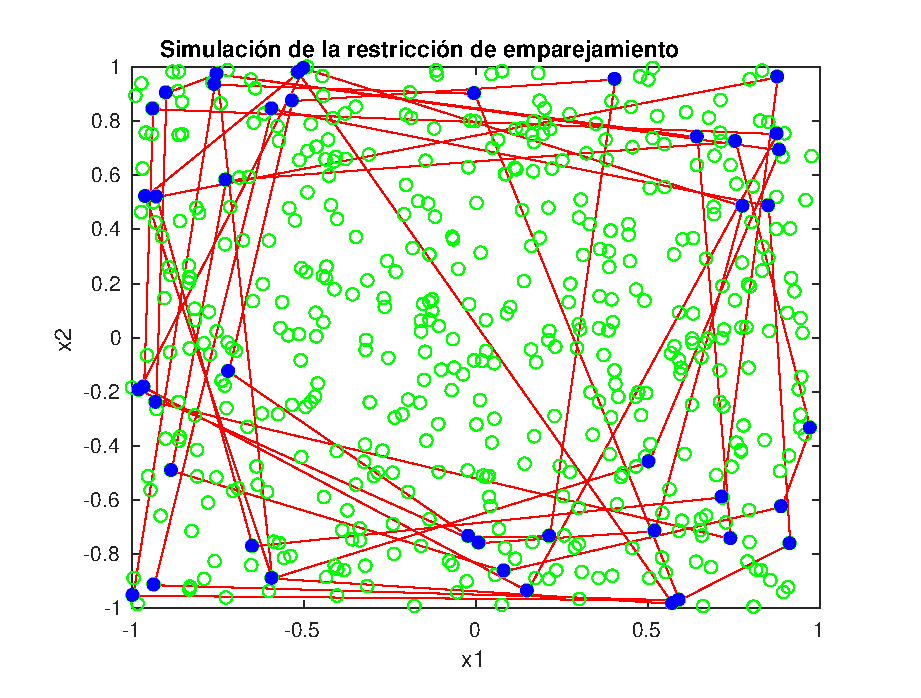
\includegraphics[scale=0.4]
{Figures_Chapter4/Mating_sample_4_points_500_gen_10.eps}
%%\decoRule
%%\label{fig:Simulacion_Mating_1}
%%\end{figure}
%%
%%\begin{figure}[H]
%%\centering
%%\scriptsize
%\includegraphics[width=6cm, height=6cm]
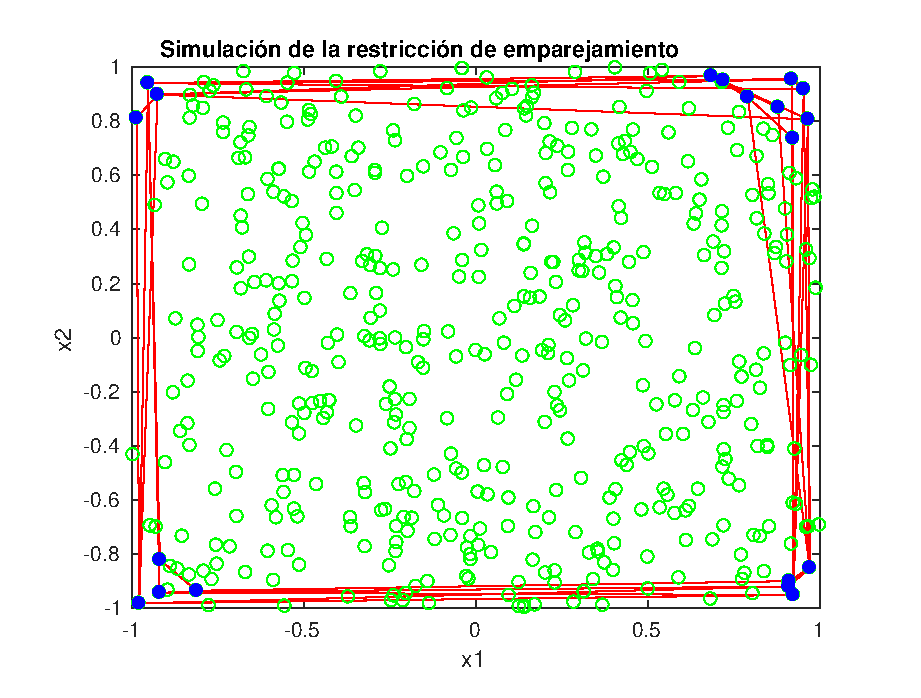
\includegraphics[scale=0.4]
{Figures_Chapter4/Mating_sample_20_points_500_gen_10.eps}
\decoRule
\caption{Simulación del proceso de emparejamiento, en la parte izquierda el tamaño de cada muestra es de 4 puntos y en la derecha de 20 puntos, se observa la tendencia de seleccionar a los individuos que corresponden al espacio factible.}
\label{fig:Simulacion_Mating}
\end{figure}

Existe la posibilidad de que con esta propuesta surgan inconvenientes de diversidad en algunos problemas de prueba, ya que este proceso de emparejamiento especial únicamente retrasa la convergencia, sin embargo en la situación especial donde las regiones subóptimas estén ubicadas en las esquinas de la región factible se tendrá un efecto de estancamiento en el proceso de búsqueda.

%%
\section{Propuesta de diversidad con elitismo especial (MOEA/D-SEBV)}

En la propuesta inicial se observa que existe una tendencia de seleccionar individuos en las esquinas del espacio de búsqueda, además aún es posible tener un efecto similar a la convergencia prematura, por lo tanto esta segunda propuesta está estructurada con el propósito de mantener la diversidad en el espacio de las variables de forma explícita.
%
En el capítulo 3 se presentó el algoritmo VSD-MOEA donde se aplica una fase de remplazo para mantener la diversidad explícitamente, en este proceso se verifica la contribución de diversidad que tiene cada individuo en el espacio de las variables por medio de la distancia al vecino más cercano, particularmente se prefieren a los individuos cuya distancia al vecino más cercano sea mayor que un umbral.
%
Conforme transcurren las generaciones este umbral es decrementado en base a un modelo lineal.
%
En base a este mismo principio se desea mantener la diversidad en esta segunda propuesta de descomposición.


El marco de referencia que corresponde al MOEA/D establecido por \citeauthor{Joel:MOEAD} fomenta un grado elevado de elitismo ya que constantemente se remplazan los individuos con mayor aptitud de cada vecindario.
%
Aunque en la literatura multi-objetivo se ha establecido que los MOEAs con propiedades elitistas proporcionan mejores resultados (\cite{Joel:Kalyanmoy}), se ha observado que es importante administrar el grado de elitismo, ya que en algunos escenarios (por ejemplo ejecuciones de largo plazo) el proceso de búsqueda puede estancarse.
%
El problema de convergencia prematura se puede observar en la figura \ref{fig:Ubicacion_Lambda} donde son considerados cuatro individuos $\{x_1, x_2, x_3, x_4\}$ y los vectores de pesos $\{ \lambda_1, \lambda_2, \lambda_3 \}$, en el proceso de actualización el individuo $x_4$ será asignado a todos los subproblemas ocasionando problemas de diversidad ya que este individuo tiene una mejor aptitud en comparación a los demás individuos, por lo tanto la población estará conformada únicamente por este individuo.
%

\begin{figure}[H]
\centering
\scriptsize
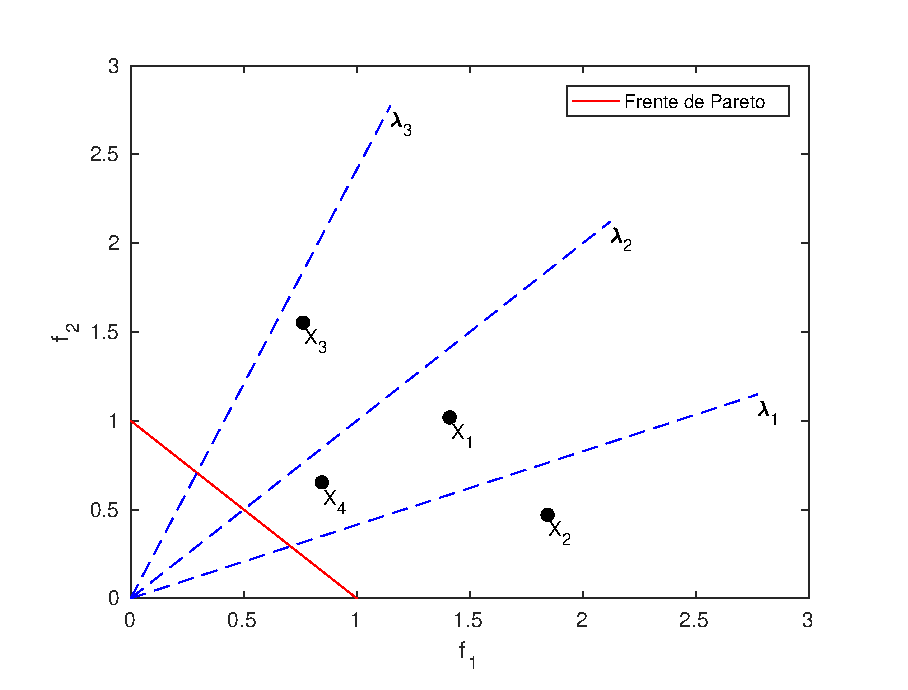
\includegraphics[scale=0.6]
{Figures_Chapter4/Lambda.eps}
\decoRule
\caption{Actualización de los subproblemas, se observa que la solución $x_4$ tendrá una mejor aptitud, por lo tanto en el clásico MOEA/D será seleccionado a todos los subproblemas ocasionando problemas de diversidad.}
\label{fig:Ubicacion_Lambda}
\end{figure}

Este inconvenientes de diversidad ya se había diagnosticado por \cite{li2009multiobjective}, quienes posteriormente propusieron el MOEA/D-DE donde se implementan dos estrategias nuevas: un número límite de veces en que un determinado individuo puede actualizar a los subproblemas y además se considera una probabilidad con la que se puede escoger a un individuo de la población entera.
%

\cite{berengueroptimizacion} explican que tanto el MOEA/D como el MOEA/D-DE buscan el óptimo a cada subproblema de forma independiente, sin embargo estos algoritmos no consideran que el individuo remplazado en un subproblema podría mejorar la solución de otro subproblema, ya que la asignación de cada subproblema se realiza buscando la mejor solución de éste, sin considerar la mejor asignación de manera global.
%
En base a estos inconvenientes sugieren transformar el proceso de selección en un problema de asignación lineal que es resuelto de forma óptima por medio del algoritmo Kuhn-Munkres.
%
La complejidad de esta propuesta es ($O(n^3)$) considerado como una debilidad, aunque es importante notar que la complejidad no incrementa de forma exponencial al aumentar el número de objetivos como es el caso del SMS-EMOA \citep{Joel:SMSEMOA}.


En esta segunda propuesta algorítmica se desea fomentar la diversidad de las soluciones evitando el remplazo inmediato de los mismos, esto se realiza agregando una fase de remplazo especial, por lo tanto es modificando el procedimiento para actualizar las soluciones vecinas de cada subproblema, en su lugar se almacenan todas las soluciones vecinas en relación a cada subproblema.
%

Así, al finalizar cada generación se implementa la fase de remplazo, donde se actualiza cada subproblema con el mejor individuo almacenado previamente, que es el individuo con mayor aptitud y cuya contribución a la diversidad en el espacio de las variables sea factible.
%
La contribución de cada individuo a la diversidad se aplica considerando la distancia al vecino más cercano entre el nuevo individuo y la población actual, por lo tanto es necesario que la diversidad aportada por el nuevo individuo sea mayor al umbral de diversidad requerido en ese momento.
%
En caso de que todos los individuos sean menores que este umbral de diversidad, se selecciona al individuo almacenado con mayor distancia al vecino más cercano induciendo así un grado mayor de diversidad.
%
En la figura \ref{fig:Actualizacion_Propuesta_2} se ilustra un ejemplo de este proceso especial de actualización, específicamente sólo se consideran dos subproblemas $\{1, 2\}$ (borde de color rojo) y a los individuos almacenados del subproblema $1 \leftarrow \{3, 4 \}$ (borde de color negro).
%
Normalmente se actualizaría el subproblema $1$ con el individuo $3$ ya que este último tiene una mejor aptitud, sin embargo dado que su contribución a la diversidad es menor que el umbral especificado (esfera punteada) se realiza la selección del individuo $4$, así se evita que el grado de diversidad sea menor en las primeras fases del algoritmo evolutivo.
%

Este procedimiento mantiene la diversidad de forma explícita, sin embargo es posible que algunos individuos con muy buena aptitud y mínima diversidad sean descartados, por lo tanto cada subproblema almacena a su individuo elite, que aunque posiblemente no participará inmediatamente en el proceso de reproducción, formará parte en el proceso de selección junto a los individuos almacenados, y posteriormente podrá ser seleccionado ya que el umbral de diversidad requerido es decrementado conforme transcurren las generaciones.

\begin{figure}[H]
\centering
\scriptsize
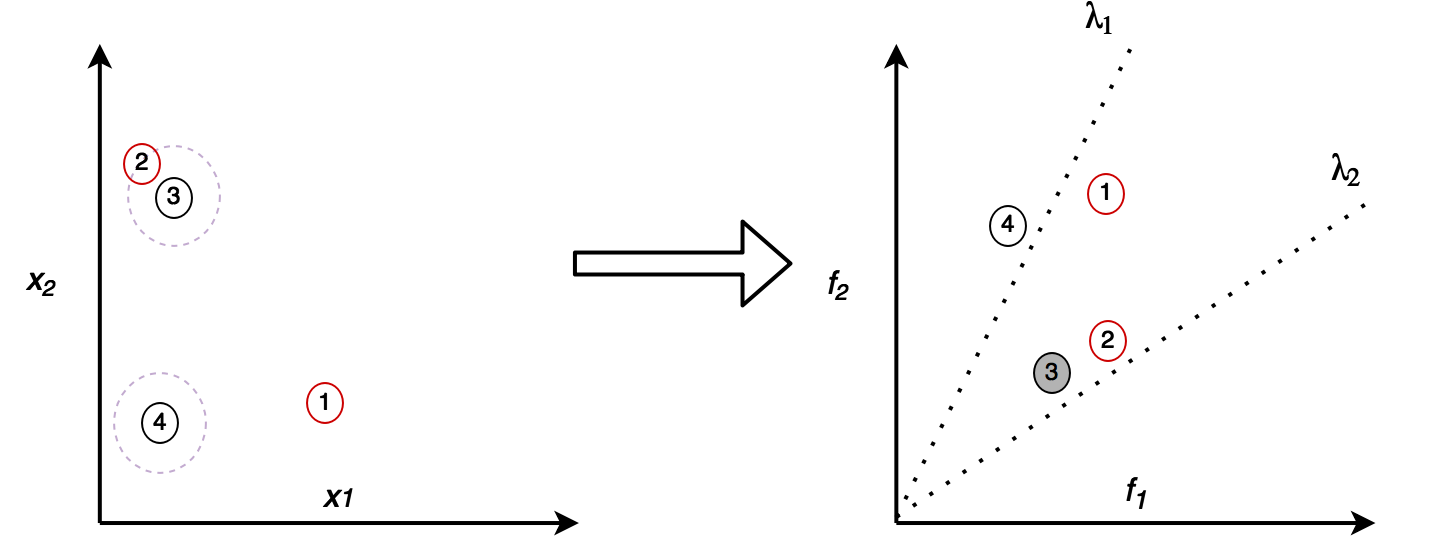
\includegraphics[scale=0.25]
{Figures_Chapter4/MOEA_SEBV.png}
\decoRule
\caption{Proceso de selección para el subproblema $1$, en la parte izquierda es el espacio de las variables y en la derecha su respectiva ubicación en el espacio objetivo. Los puntos $\{1, 2\}$ corresponden a los subproblemas actuales con borde de color rojo, en este caso únicamente se consideran a los individuos almacenados (con borde de color negro) que del subproblema $1$.}
\label{fig:Actualizacion_Propuesta_2}
\end{figure}


La propuesta de descomposición basado en diversidad con elitismo especial (MOEA/D-SEBV) se describe en el algortimo \ref{alg:MOEAD_SEBV}, donde las principales variantes del clásico MOEA/D se indican en las líneas \ref{alg:iniciar_elite}, \ref{alg:limipar_pila}, \ref{alg:almacenar_soluciones} y \ref{alg:remplazo_moea}.
%
Inicialmente los individuos elite son vacíos (línea \ref{alg:iniciar_elite}), en cada generación se realiza lo siguiente (lineas \ref{alg:iniciagen} - \ref{alg:terminagen}).
%
Se selecciona el conjunto de emparejamiento conformado por los subproblemas vecinos y globales, después de realiza la reproducción entre dos individuos seleccionados del conjunto de emparejamiento.
%
Adicionalmente se realiza la actualización del vector de referencia para realizar la evaluación del indicador.
%
Posteriormente se almacenan todos los individuos vecinos $B(i)$ de cada subproblema (línea \ref{alg:almacenar_soluciones}).
%

Una de las principiales aportaciones de esta propuesta está en la fase de remplazo (línea \ref{alg:remplazo_moea}) descrita en el algoritmo \ref{alg:Fase_Remplazo_SEBV}, donde se realiza la selección del individuo más apropiado a cada subproblema y su respectivo elite.
%
Inicialmente en la línea \ref{alg:modelo_decremento} se actualiza el umbral de diversidad mínimo permitido, el cual es decrementado en base a un modelo lineal de igual forma que el algoritmo VSD-MOEA presentado en el capítulo \ref{Chapter3}.
%
Posteriormente para cada subproblema (líneas \ref{alg:ini_for_remplazo} - \ref{alg:fin_for_remplazo}) se realiza lo siguiente.
%
Se inserta el elemento elite a la pila (línea \ref{alg:insertar_elite}), y de forma iterativa hasta que la pila del subproblema actual esté vacía (líneas \ref{alg:ini_while_remplazo_SEBV} - \ref{alg:fin_while_remplazo_SEBV}), se saca un elemento de la pila (línea \ref{alg:sacar_elemento}), se actualiza el individuo elite (línea \ref{alg:actualizar_elite}), y se actualiza al correspondiente subproblema si la diversidad del individuo nuevo es mayor al umbral $D$ y si tiene mejor aptitud (línea \ref{alg:ini_mejorar} - \ref{alg:ini_mejorar2}).
%
En el caso en que la contribución a la diversidad del individuo actual sea menor a la requerida por $D$ entonces se remplaza por el individuo nuevo que contribuya más a la diversidad (líneas \ref{alg:ini_aumentar_diversidad} - \ref{alg:fin_aumentar_diversidad}).
%


\begin{algorithm}[H]
\caption{MOEA/D-SEBV}
\label{alg:MOEAD_SEBV}
\begin{scriptsize}
\begin{algorithmic}[1]
    \STATE Inicializar los vectores de pesos $\lambda^1, \lambda^2, ..., \lambda^N$ y vecindarios $B(i)$ utilizando el enfoque tradicional del MOEA/D. \label{alg:Inicializar_Vectores_Pesos}
    \STATE Generar una población inicial de forma aleatoria $x^1, ..., x^N$.
    \STATE Inicializar $z = (z_1, ..., z_m)^T$ con un valor elevado en relación al problema. \label{alg:Inicializar_Referencia}
    \STATE $E_i \leftarrow \emptyset \forall i \in 1,...,N$ donde $E_i$ es el individuo elite del subproblema $i$. \label{alg:iniciar_elite}
  \WHILE {(no se cumpla el criterio de paro)} \label{alg:iniciagen}
    \STATE $H_i  \leftarrow \emptyset, \forall i \in 1, ..., N$ donde $H_i$ corresponde a la pila del $i-$ésimo subproblema. \label{alg:limipar_pila}
  \FOR{i=1,...,N}
    \STATE \textbf{Conjunto para emparejamiento}: Llenar aleatoriamente el conjunto de emparejamiento $P$ con los individuos $\alpha$, seleccionando cada individuo del vecindario $B(i)$ con probabilidad $\delta$ o de la población completa con probabilidad $(1 - \delta)$. \label{alg:Emparejamiento}
    \STATE \textbf{Reproducción}: Seleccionar a dos individuos del conjunto de emparejamiento e implementar los operadores de reproducción para generar a nuevos individuos (y). 
    \STATE \textbf{Actualizar el vector de referencia $z$}: Para cada j = 1,..,m, si $z_j > f_j(y)$, entonces asignar $z_j = f_j(y)$.
    \STATE \textbf{Actualizar las soluciones vecinas}: Para cada índice $j \in B(i)$, meter a la pila $H_j(y)$. \label{alg:almacenar_soluciones}
    \ENDFOR
    \STATE \textbf{Fase de remplazo}: Para todo subproblema $i \in 1, ..., N$ seleccionar al mejor individuo de $H_i$ y actualizar al elite $E_i$. \label{alg:remplazo_moea}
  \ENDWHILE \label{alg:terminagen}
\end{algorithmic}
\end{scriptsize}
\end{algorithm}


\begin{algorithm}[H]
\algsetup{linenosize=\tiny}
  \scriptsize
	\caption{Fase de remplazo MOEA/D-SEBV} 
	\begin{algorithmic}[1]
    	\STATE Entrada: $P^t$ (El conjunto de subproblemas), $H$ (Los individuos almacenados de cada subproblema), $E$ (El conjunto de individuos elite de cada subproblema)
    	\STATE Salida: $P^{t+1}$
		\STATE $D = D_I - D_I *2* \frac{G_{Transcurridas}}{G_{Final}}$ \label{DInicial}	\label{alg:modelo_decremento}
	\FOR{i=1, ..., N} \label{alg:ini_for_remplazo}
	     \STATE Meter a la pila $H(E_i)$ \label{alg:insertar_elite}
	     \STATE $DCN(P_i^t) =  $ Distancia al Vecino más Cercano($P_i^t$) \Comment{ Calcular la contribución a la diversiad de $P_i^t$ en la población }
	   \WHILE{$H_i$ no este vacío} \label{alg:ini_while_remplazo_SEBV}
	      \STATE $C_i$ = sacar($H_i$) \label{alg:sacar_elemento}
	      \STATE $DCN(C_i) = $Distancia al Vecino más Cercano($C_i$, $P_i^t$) \Comment{ Calcular la contribución a la diversiad de $t_i$ en lugar de $P_i^t$ }
	      \STATE $E_i$ = $C_i$ si $g(C_i| \lambda^i, z) < g(E_i| \lambda^i, z)$  \label{alg:actualizar_elite}
    %\STATE \textbf{Actualizar las soluciones vecinas}: Para cada índice $j \in B(i)$, si $g(y| \lambda^j, z) < g(x_j| \lambda^j, z)$, entonces asignar $x^j = y$.\label{alg:Actualizar_Vecindarios}
	      \IF{   $ DCN(C_i) \geq$ D} \label{alg:ini_mejorar}
	         \STATE $P_i^t$ = $C_i$ si $g(C_i| \lambda^i, z) < g(P_i^t| \lambda^i, z)$ \label{alg:ini_mejorar2}
	      \ELSIF{  $DCN(P_i^t)< D$ } \label{alg:ini_aumentar_diversidad}
		\IF{ $DCN(C_i) > DCN(P_i^t)$   }
		 \STATE Meter a la pila $H( P_i  )$
		 \STATE $P_i = C_i$
		\ENDIF \label{alg:fin_aumentar_diversidad}
	      \ENDIF
	   \ENDWHILE \label{alg:fin_while_remplazo_SEBV}
	\ENDFOR \label{alg:fin_for_remplazo}
    \label{alg:Fase_Remplazo_SEBV}
\end{algorithmic}
\end{algorithm}

%%%%\subsection{Trayectorias MOEA/D-SEBV}
%%%%
%%%%Para analizar el comportamiento de la diversidad inducida en esta segunda propuesta, se realizó una simulación en donde se resuelve la instancia UF5, como se puede observar en el capítulo \ref{Chapter2} el conjunto óptimo esta conformado por puntos en el espacio de las variables que a su vez corresponde a 21 puntos del frente de Pareto, particularmente esta instancia de considera difícil ya que es difícil ya que existe una pérdida de diversidad considerable al permitir que una solución sea asignada a varios subproblemas, teniendo como resultado varias réplicas.
%%%%
%%%%%%Trayectoria de un vector de pesos del MOEA/D sin diversidad explícita


\subsection{Observaciones}

Esta propuesta posee la ventaja de fomentar la diversidad explícitamente, además si el umbral de diversidad inicial es muy elevado, entonces el proceso evolutivo consistirá en maximar la distancia al vecino mas cercano de cada individuo, ubicando a los puntos de forma bien distribuida en el espacio factible.
%
Por lo tanto en el proceso de búsqueda únicamente se reemplazarán los individuos cuya contribución a la diversidad sea estrictamente mayor al umbral de diversidad de ese momento.
%
En esta propuesta ya no es necesario indicar un límite de actualizaciones como es implementado en el MOEA/D-DE, por otra parte si es necesario asignar la diversidad inicial que se desea del espacio de búsqueda.


Aunque esta propuesta promueve la diversidad de forma explícita, existe un inconveniente con este esquema, ciertos subproblemas pueden no ser actualizados durante varias generaciones al no encontrar soluciones mejores, por lo tanto la capacidad de exploración dependerá principalmente por los individuos a emparejar y los operadores, ya que si siempre se emparejan los mismos padres existe una tendencia a generar individuos en las mismas regiones.
%
Así, en el peor de los casos si al inicio de la ejecución se asigna una solución a un subproblema y esta solución pertenece a una región suboptima, entonces esta solución no será actualizada durante muchas generaciones hasta encontrar otra solución con mejor aptitud, lo cual en algunas situaciones puede ser muy problemático.
%

Este esquema provoca que los subproblemas sean actualizados de forma muy agresiva, ya que un indiviuo puede permanecer asignado a un subproblema durante varias generaciones hasta que sea reemplazado por otro individuo, este reemplazo puede provocar grandes desplazamientos en el espacio factible y por lo tanto las zonas promisorias pueden ser ignoradas, particularmente este comportamiento es considerado como una desventaja en el proceso de búsqueda.
%

\section{Algoritmo de descomposición basado en la diversidad (VSD-MOEA/D)}

El MOEA/D-SEBV es considerado como uno de los primeros MOEAs basados en descomposición que promueven la diversidad explícitamente considerando el criterio de paro.
%
Como ya se comentó anteriormente este algoritmo posee algunas desventajas al promover la diversidad de forma explícita, principalmente por el hecho de que la diversidad es considerada de forma independiente en cada subproblema, proporcionando como resultado diversidad no efectiva (\cite{Joel:mahfoud1995niching}).
%
En base a esto se propone el VSD-MOEA/D que a diferencia del MOEA/D-SEBV se considera la diversidad de forma global, específicamente esto es realizado en la fase de remplazo donde es implementado el principio de especiación (\cite{yang2017multimodal}, \cite{gao2014cluster}) que es utilizado en el área de optimización multimodal.
%
Adicionalmente se utiliza una población de individuos elite los cuales son actualizados inmediatamente después de la reproducción, que a diferencia del MOEA/D clásico donde son actualizados los individuos padre de la siguiente generación.
%
Posteriormente, la población de individuos elite participan en la especiación que es parte de la fase de remplazo, de esta forma son gradualmente introducidos los individuos elite en el proceso de búsqueda.
%

\subsection{Especiación de la población}

Particularmente, el procedimiento de especiación asocia a los individuos en base a su respectivas distancias (\cite{li2005efficient}), por lo tanto de forma iterativa se seleciona una semilla y se asocian todos los individuos de esa especie como se indica en la ecuación (\ref{eq:especiacion}), donde $S_i$ es la $i-$ésima especie, $P$ es la población, $x_i$ es el individuo a relacionar con su respectiva semilla y $r$ es el radio de las especies.
%
\begin{equation}\label{eq:especiacion}
\begin{split}
S_i = \left \{ x_j | x_j \in P \quad y \quad dist(x_{semilla}, x_j) = \sqrt{ \sum_{d=1}^D ( x_{semilla}^d - x_j^d )  } \leq r \right \}
\end{split}
\end{equation} 

%
El procedimiento de especiación es descrito en el algoritmo \ref{alg:Especiacion}, donde inicialmente se ordenan los individuos en base a su aptitud (línea \ref{alg:Ordenar_especiacion}), luego de forma iterativa se realiza lo siguiente.
%
Se considera al mejor individuo como una semilla (línea \ref{alg:seleccion_semilla}) y los individuos relacionados a esta semilla son removidos del conjunto $P$ (línea \ref{alg:remover_especiacion}), así se repite este proceso hasta que no existan individuos en la población $P$.
%
\begin{algorithm}[H]
\scriptsize
\caption{Clusterización con especiación}
\label{alg:Especiacion}
\begin{scriptsize}
\begin{algorithmic}[1]
\STATE Entrada: Población $P$ con $N$ individuos,  radio de la especie $r$.
\STATE Ordenar a $P$ de acuerdo a su aptitud. \label{alg:Ordenar_especiacion}
\WHILE{P no esté vacío}
   \STATE El mejor individuo es seleccionado como semilla para crear una nueva especie. \label{alg:seleccion_semilla}
   \STATE Encontrar a otros individuos de esta especie de acuerdo a la ecuación \ref{eq:especiacion}.
   \STATE Remover de $P$ todos los individuos de esta especie.\label{alg:remover_especiacion}
\ENDWHILE
\end{algorithmic}
\end{scriptsize}
\end{algorithm}

Es importante señalar que este procedimiento es utilizado en el VSD-MOEA/D para introducir a los individuos que pertenecen al conjunto elite, por lo tanto si existen individuos muy similares en el conjunto elite se seleccionará únicamente una semilla y los demás individuos serán descartados.
%
En la figura \ref{fig:Especiation} se puede observar el principio de especiación considerando únicamente una dimensión y su respectiva aptitud, donde se elige primero a la semilla $S_1$ y se eliminan a los individuos con una distancia menor al radio de la especie $r$, luego se escoge a la segunda mejor semilla $S_2$ y se realiza este mismo procedimiento. 
\begin{figure}[H]
\centering
\scriptsize
%\includegraphics[width=6cm, height=6cm]
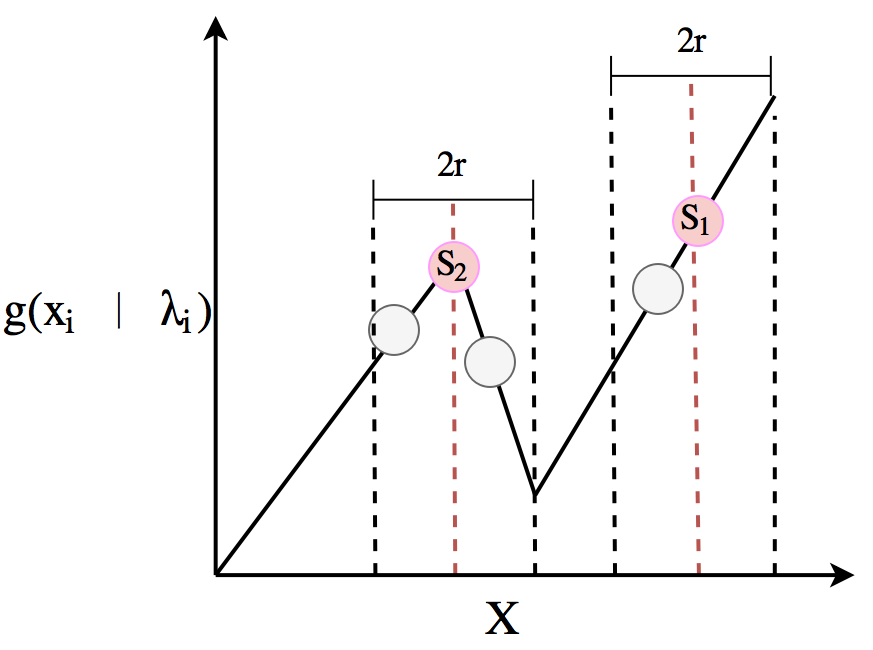
\includegraphics[scale=0.2]
{Figures_Chapter4/Especiacion.png}
\decoRule
\caption{Selección de dos semillas $S_1$ y $S_2$, considerando la aptitud de su respectivo subproblema $\lambda_i$}
\label{fig:Especiation}
\end{figure}


%
\subsection{Propuesta algorítmica VSD-MOEA/D}

El proceso involucrado en cada generación es descrito en la figura \ref{fig:Proceso_Generacion_VSD-MOEA_D}, en la selección se llena un conjunto de emparejamiento, de donde se escogeran los individuos padre que se reproducirán, posteriormente se realiza la actualización de la población elite y al final se únen las tres poblaciones de donde se seleccionará el conjunto de padres de la siguiente generación.

\begin{figure}[H]
\centering
\scriptsize
%\includegraphics[width=6cm, height=6cm]
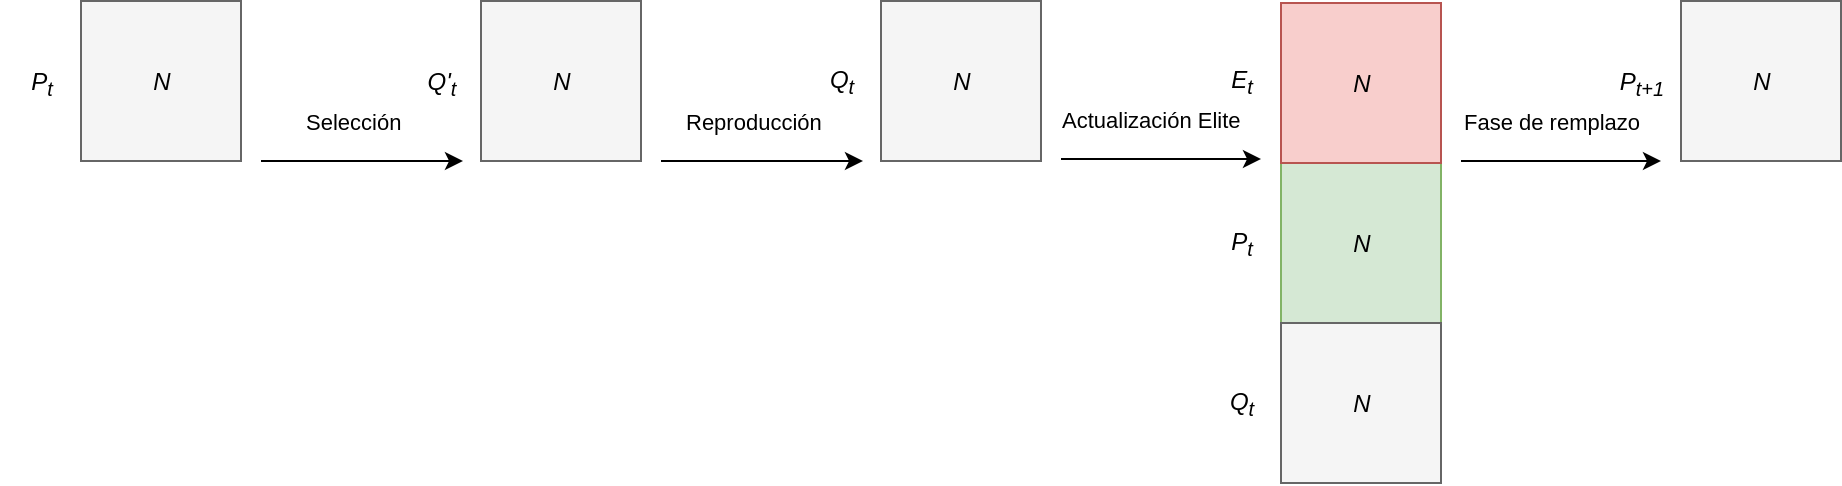
\includegraphics[scale=0.2]
{Figures_Chapter4/Evolution_Process_Decomposition.png}
\decoRule
\caption{Proceso para seleccionar una población $P_{t+1}$ y generar una población nueva $Q_{t+1}$  en cada generación.}
\label{fig:Proceso_Generacion_VSD-MOEA_D}
\end{figure}


El procedimiento principal del VSD-MOEA/D es mostrado en el algoritmo \ref{alg:VSD_MOEAD}, donde primeramente se inicializan los vectores de pesos mediante un método generador (previamente explicado) y se construyen los vecindarios en base a las distancias entre los vectores de pesos (línea \ref{alg:Inicializacion_VSD_MOEAD}).
%
Luego se genera la población inicial de forma aleatoria dentro de los límites del espacio de búsqueda y se inicializa el vector de referencia (líneas \ref{alg:generar_poblacion_MOEAD} - \ref{alg:Inicializar_Referencia_MOEAD}).
%
Así en cada generación se realiza el siguiente proceso.
%
Se selecciona el conjunto de emparejamiento que corresponden a los individuos padre (línea \ref{alg:Emparejamiento_MOEAD}).
%
Posteriormente, en base a los individuos seleccionados para emparejase se implementa el proceso de reproducción mediante los operadores evolutivos (línea \ref{alg:reproduccion_MOEAD}), normalmente se utiliza DE y/o operadores genéticos (SBX, mutación polinomial), es importante analizar el comportamiento de los operadores a utilizar con este esquema de diversidad.
%

La actualización de cada subproblema (línea \ref{alg:actualizar_elite_MOEAD}) es aplicado únicamente a la población elite, con el objetivo de evitar la convergencia prematura.
%
Al final de cada generación (linea \ref{alg:remplazo_MOEAD}) se aplica la fase de remplazo indicado en el algoritmo \ref{alg:Fase_Remplazo_VSD-MOEAD}, el cual funciona de la siguiente forma.
%
Inicialmente se calcula el radio de las especies (linea \ref{alg:especies_radio}) que representa el grado de diversidad que se desea promover.
%
Posteriormente, se combinan los individuos hijo, padres y elite, que son almacenados en una población temporal $R_t$ (línea \ref{alg:union_MOEAD}).
%
En la línea \ref{alg:ordenacion_moead}, en base a su aptitud e incrementalmente se ordenan a los individuos que pertenecen a $R_t$.
%
El proceso de especiación es aplicado a la población $R_t$ (líneas \ref{alg:especiacion_ciclo_ini} - \ref{alg:especiacion_ciclo_fin}) donde se eligen los individuos que corresponden a las semillas factibles, es importante notar que si el radio de cada especie es muy elevado entonces únicamente se elegirá a una semilla, en el caso contrario donde el radio sea mínimo, entonces el número de semillas estará conformado por el número de subproblemas.
%

\begin{figure}[]
\centering
\scriptsize
%\includegraphics[width=6cm, height=6cm]
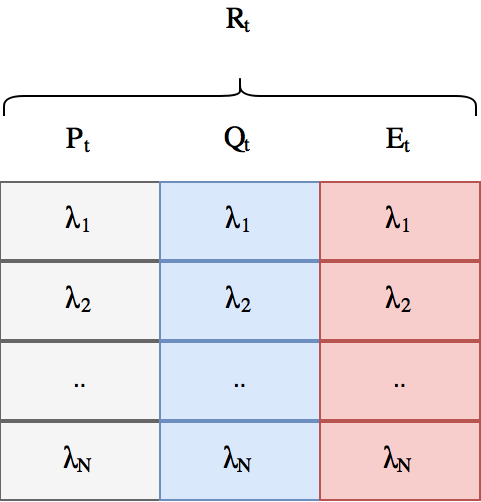
\includegraphics[scale=0.3]
{Figures_Chapter4/Related_Populations.png}
\decoRule
\caption{Cada subproblema está relacionado a tres individuos en $R_t$ que está conformado por los padres $P_t$, hijos $Q_t$ y elite $E_t$.}
\label{fig:subproblems_populations}
\end{figure}


Así, cada vez que se seleccione un subproblema como semilla los demás individuos relacionados a ese subproblemas serán desactivados, por lo tanto ya no participarán como parte del proceso de especiación.
%
Al terminar este proceso de especiación pueden existir subproblemas sin asignar, por lo tanto se seleccionan los individuos de los subproblemas del conjunto $Penalizado$ cuya contribución a la diversidad hacia $P_{t+1}$ sea mayor, para calcular la contribución se sugiere utiliza la distancia al vecino más cercano.
%
Es importante notar que al seleccionar un individio del conjunto $Penalizado$ se eliminarán a los individuos relacionados con el subproblema asignado.

\begin{algorithm}[H]
\caption{VSD-MOEA/D}
\label{alg:VSD_MOEAD}
\begin{scriptsize}
\begin{algorithmic}[1]
    \STATE Inicializar los vectores de pesos $\lambda^1, \lambda^2, ..., \lambda^N$ y vecindarios $B(i)$ utilizando el enfoque tradicional del MOEA/D. \label{alg:Inicializacion_VSD_MOEAD}
    \STATE Generar una población inicial de forma aleatoria $x^1, ..., x^N$. \label{alg:generar_poblacion_MOEAD}
    \STATE Inicializar $z = (z_1, ..., z_m)^T$ con un valor elevado en relación al problema. \label{alg:Inicializar_Referencia_MOEAD}
    \STATE $E \leftarrow \emptyset$
    \STATE $Q \leftarrow \emptyset$
    \STATE $t = 0$
  \WHILE {(no se cumpla el criterio de paro)} \label{alg:iniciagen}
  \FOR{i=1,...,N}
    \STATE \textbf{Conjunto para emparejamiento}: Utilizar a $P_t$ para llenar aleatoriamente el conjunto de emparejamiento $M$ con los individuos $\alpha$, seleccionando cada individuo del vecindario $B(i)$ con probabilidad $\delta$ o de la población completa con probabilidad $(1 - \delta)$. \label{alg:Emparejamiento_MOEAD}
    \STATE \textbf{Reproducción}: Aplicar los operadores de reproducción a los individuos del conjunto de emparejamiento $M$ para generar a la población hijo $Q_{t,i}$. \label{alg:reproduccion_MOEAD}
    \STATE \textbf{Actualizar el vector de referencia $z$}: Para cada j = 1,..,m, si $z_j > f_j(Q_{t,i})$, entonces asignar $z_j = f_j(Q_{t,i})$.
    \STATE \textbf{Actualizar las soluciones vecinas}: Para cada índice $j \in B(i)$, $E_{t,j}$ = $Q_{t,i}$ si $g( Q_{t,i}| \lambda^j, z) < g(E_{t,j} | \lambda^j, z)$  \label{alg:actualizar_elite_MOEAD}.
    \ENDFOR
    \STATE \textbf{Fase de remplazo}: Seleccionar $P_{t+1}$ de $P_t \cup Q_t \cup E_t$. \label{alg:remplazo_MOEAD}
    \STATE $t = t + 1$
  \ENDWHILE \label{alg:terminagen}
\RETURN{$P_{t+1}$}
\end{algorithmic}
\end{scriptsize}
\end{algorithm}


\begin{algorithm}[H]
\algsetup{linenosize=\tiny}
  \scriptsize
	\caption{Fase de remplazo VSD-MOEA/D} 
	\begin{algorithmic}[1]
	\STATE Entrada: Población $P_t$ (Población de la generación actual), $Q_t$ (Población hijo), $E_t$ (Población elite).
	\STATE Salida: $P_{t+1}$
	\STATE Definir el radio de las especies como $D = D_I - D_I *2* \frac{G_{Transcurridas}}{G_{Final}}$ \label{alg:especies_radio}
	\STATE $P_{t+1} = \emptyset$
	\STATE $Penalizados = \emptyset$
	\STATE $R_t = P_t \cup Q_t \cup E_t$ \label{alg:union_MOEAD}
	\STATE Ordenar a $R_t$ de acuerdo a su aptitud. \label{alg:ordenacion_moead} \tikzmark{top}
	\WHILE{ $R_t$ no esté vacío OR $|P_{t+1}| < N$} \label{alg:especiacion_ciclo_ini}
	   \STATE El mejor individuo es seleccionado como semilla para crear una nueva especie.
	   \STATE Encontrar a otros individuos de esta especie de acuerdo a la ecuación \ref{eq:especiacion}.
	   \STATE mover de $P$ a $Penalizados$ todos los individuos que corresponden a esta especie.\tikzmark{right}
	\ENDWHILE \label{alg:especiacion_ciclo_fin} \tikzmark{bottom}
	\STATE $Penalizados = Penalizados \ E_t $, remover del conjunto $Penalizados$ a todos los individuos que estén en el conjunto Elite $E_t$.
	\WHILE{ $|P_{t+1}| < N$}
	   \STATE   Mover de $Penalizados$ a $P_{t+1}$ al individuo que tenga mayor contribución a la diversidad en el espacio de la variables.
	\ENDWHILE
	\RETURN{$P_{t+1}$}
    \label{alg:Fase_Remplazo_VSD-MOEAD}
\AddNote{top}{bottom}{right}{En esta sección es implementado la especiación.}
\end{algorithmic}
\end{algorithm}

\subsection{Observaciones}

En esta propuesta, se consideran tres poblaciones en la fase de reemplazo, en consecuencia es analizada la diversidad una forma global.
%
Es importante analizar el efecto de los operadores a utilizar con los esquemas de diversidad, ya que al promover individuos bien distribuidos en el espacio de búsqueda, dependiendo del operador, puede existir una tendencia negativa en el proceso de búsqueda, por ejemplo, generar soluciones fuera del espacio factible.
%

En esta tercera propuesta no es necesario indicar el número de veces en que una solución puede reemplazar a los subproblemas vecinos, como es realizado en el MOEA/D-DE, pero en caso de que este parámetro sea indicado, dependiendo del problema, el grado de diversidad será elevado, y por lo tanto podrían existir problemas de convergencia al frente Pareto.
%

Por otra parte, el tamaño de las vecindades afectan el proceso de búsqueda, así una vecindad pequeña resulta en explorar regiones más específicas del espacio de búsqueda, en contraparte una vecindad grande provoca el emparejamiento de individuos de cualquier región en el espacio de búsqueda.
%
Por lo tanto, en este esquema, el tamaño de las vecidades influye en las regiones donde se desea inducir un grado de diversidad, esto a largo plazo provoca un desempeño muy similar al pardigma de EAs paralelos.
%


\section{Complejidad de los algoritmos propuestos }

En esta sección se presenta la complejidad de las tres propuestas algorítmicas que pertenecen a este capítulo.
%
Para la estimación de cada complejidad únicamente se discuten las secciones cuyo grado de complejidad sea diferente al MOEA/D que es $O(MNT)$, donde $M$ es el número de objetivos, $N$ es el número de subproblemas y $T$ es el tamaño de cada vecindad, aunque en el MOEA/D-DE existe un parámetro que indica número máximo de veces que un individuo puede actualizar a otro vecindario, aquí se considera el peor caso donde se actualizan todas las vecindades de un subproblema.
%
Específicamente la complejidad del MOEA/D es dominada en el proceso donde se actualizan los subproblemas ya que para cada subproblema se realizan $T$ comparaciones.
%
En el MOEA/D-EVSD (algoritmo \ref{alg:MOEAD_EVSD}) en cada generación se considera llenar un conjunto de emparejamiento con tamaño $\alpha$ en la línea 6, posteriormente en la línea 7 se seleccionan a los dos individuos más alejados, por lo tanto se realizan $\alpha(\alpha-1)$ comparaciones.
%
Entonces la complejidad del MOEA/D-EVSD es $O(MNT + \alpha^2N)$, este orden puede ser dominado por el tamaño de la vecindad.
%

En la segunda propuesta MOEA/D-SEBV (algoritmo \ref{alg:MOEAD_SEBV}) se consideran dos secciones críticas para el cálculo de la complejidad: La actualización de las soluciones vecinas (línea 11) y la fase de remplazo (línea 12).
%
Para realizar la actualización de las soluciones vecinas en cada subproblema se insertan $T$ elementos a la pila, por lo tanto para cada generación se iteran $NT$.
%
El grado de complejidad de la fase de remplazo es indicado en el algoritmo \ref{alg:complejidad_MOEAD_SEBV}, específicamente en las líneas 6 y 9 se revisa la contribución a la diversidad de cada elemento, por lo tanto para cada subproblema se verifican $T$ elementos y con el elite $H=T+1$.
%
Para obtener la contribución a la diversidad de un individuo se realizan $N-1$ comparaciones, $N(N-1)$ en la línea 6 y $N(N-1)(H)$ en la línea 9.

También en este proceso de remplazo se puede considerar la actualización del individuo elite (línea 10) que consiste de $MNH$ pero el cálculo de la complejidad dominantes corresponde en calcular la contribución de diversidad de cada individuo a la población.
%
Por lo tanto, considerando el costo de cada línea se estima la complejidad:
\begin{equation}
\begin{split}
T(N) &= c_1 + c_2N + c_3N + c_4(N)(N-1) + c_5NH + c_6NH + c_7HN(N-1) +c_8HMN + \sum_{k=8}^{15} c_k(NH) \\
    &=  c_1 + N(c_2 + c_3 - c_4) + N H \sum_{k=5}^{15} c_k + N^2c_4+ HMNc_8 + H N^2 c_7
\end{split}
\end{equation}
%
Considerando los términos dominantes se estima que la cota superior MOEA/D-SEBV:
\[
    T(N,M,H)= 
\begin{cases}
     O(HNM),& \text{si} M > N\\
     O(HN^2),& \text{de otra forma}
\end{cases}
\]
Generalizando y considerando que existe un menor número de objetivos que individuos la complejidad en el peor caso es $O(HN^2)$, donde si el tamaño de la vecindad es el número de subproblemas ($T=N$) se estima la cota superior, es decir el peor caso como $O(N^3)$.

\begin{algorithm}[H]
%\algsetup{linenosize=\tiny}
  \scriptsize
	\caption{Fase de remplazo MOEA/D-SEBV - Complejidad} 
        \label{alg:complejidad_MOEAD_SEBV}
	\begin{algorithmic}[1]
    	\STATE Entrada: $P^t$ (El conjunto de subproblemas), $H$ (Los individuos almacenados de cada subproblema), $E$ (El conjunto de individuos elite de cada subproblema)
    	\STATE Salida: $P^{t+1}$
         \algcost{\textit{Costo}}{\textit{Iteraciones}}
		\STATE $D = D_I - D_I *2* \frac{G_{Transcurridas}}{G_{Final}}$\algcost{$c_1$}{$1$}
	\FOR{i=1, ..., N} \algcost{$c_2$}{$N$}
	     \STATE Meter a la pila $H(E_i)$\algcost{$c_3$}{$N$}
	     \STATE $DCN(P_i^t) =  $ Distancia al Vecino más Cercano($P_i^t$) \algcost{$c_4$}{$N(N-1)$}
	   \WHILE{$H_i$ no este vacío} \algcost{$c_5$}{$ N H $}
	      \STATE $C_i$ = sacar($H_i$) \algcost{$c_6$}{$N H$}
	      \STATE $DCN(C_i) = $Distancia al Vecino más Cercano($C_i$, $P_i^t$) \algcost{$c_7$}{$N H (N-1)$}
	      \STATE $E_i$ = $C_i$ si $g(C_i| \lambda^i, z) < g(E_i| \lambda^i, z)$  \algcost{$c_8$}{$N H M$}
	      \IF{   $ DCN(C_i) \geq$ D}  \algcost{$c_9$}{$N H $}
	         \STATE $P_i^t$ = $C_i$ si $g(C_i| \lambda^i, z) < g(P_i^t| \lambda^i, z)$ \algcost{$c_{10}$}{$N H$}
	      \ELSIF{  $DCN(P_i^t)< D$ }  \algcost{$c_{11}$}{$N H $}
		\IF{ $DCN(C_i) > DCN(P_i^t)$ } \algcost{$c_{12}$}{$N H $}
		 \STATE Meter a la pila $H( P_i  )$ \algcost{$c_{13}$}{$N H $}
		 \STATE $P_i = C_i$ \algcost{$c_{15}$}{$N H $}
		\ENDIF 
	      \ENDIF
	   \ENDWHILE 
	\ENDFOR 
\end{algorithmic}
%%\AddNote{top}{bottom}{right}{We loop here until $r=0$.} %\tikzmark{top}
%%\AddNote{top}{bottom}{right2}{We loop here until $r=0$.}
%%\AddNote{top}{bottom}{right3}{We loop here until $r=0$.}
\end{algorithm}


%
Finalmente, en la última propuesta VSD-MOEA/D (algoritmo \ref{alg:VSD_MOEAD}) la sección que influye más en la estimación de la complejidad es la fase de remplazo (línea 13).
%
El costo de cada instrucción en la fase de remplazo está indicado en el algoritmo \ref{alg:Fase_Remplazo_VSD-MOEAD_complejidad}, donde primeramente se mueven todos los individuos al conjunto $R_t$ haciendo $3N$ iteraciones, después de eso se ordenan incrementalmente los $R_t$ individuos de acuerdo a su aptitud, realizando $3NM log(3NM)$ iteraciones por el algoritmo de ordenamiento.
%
Posteriormente en las líneas 8 - 11 se define el procedimiento de especiación donde el peor caso es cuando cada subproblema representa una especie.
%
La estimación de esta parte se realiza por medio de inducción, considerando el peor caso donde todos los individuso pueden ser una semilla ($3N$ especies), así cada vez que se elige una especie se desactiva el subproblema relacionado y se mueven al conjunto de penalizados los otros dos individuos relacionados a ese subproblema.
%
Inicialmente al tomar una la primera semilla son realizadas $3N-3$ comparaciones, luego en la segunda semilla son $3N-6$ iteraciones, este procedimiento se realiza hasta que el número de semillas sea igual a $N$, $\{3N-3, 3N-6, 3N-9,..., 3N-3i \}$
%
Por lo tanto la estimación de la especiación ( \cite{cormen2009introduction} ) es:
\begin{equation}
\sum_{i=1}^N 3N-3i = 3N^2 - 3 \sum_{i=1}^N i = \frac{3N^2}{2} - \frac{3N}{2}
\end{equation}

Así el procedimiento de especiación en el peor caso se realizan $\frac{3N^2}{2} - \frac{3N}{2}$ iteraciones.
%
Entonces si todos los subproblemas son considerados como una especie no existirán individuos penalizados, por lo tanto las líneas 12 - 14 no afectarían el rendimiento del algoritmo.
%
Por otra parte en el caso en que únicamente exista una sola especie a causa de que el radio sea muy elevado, también se puede calcular de forma inductiva.
%
Primeramente, existirán $2N-2$ individuos penalizados (es $2N$ debido a que no se considera el conjunto elite), entonces en la primer iteración se realizan $1(2N-2)$ para encontrar al individuo con mayor distancia al vecino más cercano, en la segunda es $2(2N-4)$, entonces de forma iterativa se tiene $\{ i(2N-2i) \}$, por lo tanto la estimación de esta parte es:

\begin{equation}
\begin{split}
\sum_{i=1}^N i(2N-2i) = \frac{2N^2(N+1)}{2} - \frac{1}{6} N(N+1)(2N+1) = \frac{N^3}{3} - \frac{N}{3}
\end{split}
\end{equation}
%%
Por lo tanto considerando el costo de cada sección de la fase de remplazo se estima la cota superior como:
\begin{equation}
\begin{split}
T(N, M) =&
      c_1 + c_2 + c_3 3N + c_4 3NM log(3NM)+ c_5 N + c_6 +  c_7  \left ( \frac{3N^2}{2} - \frac{3N}{2} \right ) \\ 
	&+  c_8 N + c_9 N + c_{10} N + c_{11} \left ( \frac{N^3}{3} - \frac{N}{3} \right ) \\
=&  c_1 + c_2 + c_6 + N \left ( 3 c_3 + c_5 + c_8 + c_9 + c_{10} + \frac{3 c_7}{2} - \frac{c_{11}}{3} \right ) \\
	&+ (NM log(NM))(3 c_ 4) + N^2(\frac{3 c_7}{2}) + N^3 \frac{c_{11}}{3}
\end{split}
\end{equation}
Considerando los terminos dominantes se estima que la complejidad en el peor caso del VSD-MOEA/D es $O(N^3)$.
%
La sección que puede afectar más el rendimiento del algoritmo es cuando la cantidad de individuos penalizados es significativa, es decir cuando el radio de las especies es elevada, sin embargo esto sucederá únicamente al inicio del algoritmo, y posteriormente cambiará la complejidad a $O(N^2)$.
%
Específicamente el cálculo del vecino más cercano influye directamente en la complejidad, entonces optimizar este método ya sea con alguna estrategia de geometría computacional o algún método estocástico, puede disminuir un grado en la complejidad del algoritmo.

\begin{algorithm}[H]
\algsetup{linenosize=\tiny}
  \scriptsize
	\caption{Fase de remplazo VSD-MOEA/D - Complejidad}
         \label{alg:Fase_Remplazo_VSD-MOEAD_complejidad}
	\begin{algorithmic}[1]
	\STATE Entrada: Población $P_t$ (Población de la generación actual), $Q_t$ (Población hijo), $E_t$ (Población elite).
	\STATE Salida: $P_{t+1}$ \algcost{\textit{Costo}}{\textit{Iteraciones}}
	\STATE Definir el radio de las especies como $D = D_I - D_I *2* \frac{G_{Transcurridas}}{G_{Final}}$ 
	\STATE $P_{t+1} = \emptyset$ \algcost{$c_{1}$}{$1$}
	\STATE $Penalizados = \emptyset$ \algcost{$c_{2}$}{$1$}
	\STATE $R_t = P_t \cup Q_t \cup E_t$ \algcost{$c_{3}$}{$3N$}
	\STATE Ordenar a $R_t$ de acuerdo a su aptitud.  \algcost{$c_{4}$}{$3NM log(3NM)$}
	\WHILE{ $R_t$ no esté vacío OR $|P_{t+1}| < N$} \algcost{$c_{5}$}{$N$}
	   \STATE El mejor individuo es seleccionado como semilla para crear una nueva especie. \algcost{$c_{6}$}{$1$}
	   \STATE Encontrar a otros individuos de esta especie de acuerdo a la ecuación \ref{eq:especiacion} \algcost{$c_{7}$}{$\frac{3N^2}{2} - \frac{3N}{2}$}
	   \STATE mover de $P$ a $Penalizados$ todos los individuos que corresponden a esta especie.\algcost{$c_{8}$}{$N$}
	\ENDWHILE 
	\STATE $Penalizados = Penalizados \notin E_t $, remover del conjunto $Penalizados$ \par
		\hskip\algorithmicindent a todos los individuos que pertenezcan al conjunto Elite $E_t$.\algcost{$c_{9}$}{$N$}
	\WHILE{ $|P_{t+1}| < N$} \algcost{$c_{10}$}{$N$}
	   \STATE   Mover de $Penalizados$ a $P_{t+1}$ al individuo que tenga mayor contribución \par
	 \hskip\algorithmicindent a la diversidad en el espacio de la variables. \algcost{$c_{11}$}{$\frac{N^3}{3} - \frac{N}{3}$}
	\ENDWHILE \\

	\RETURN{$P_{t+1}$}
\end{algorithmic}
\end{algorithm}

\begin{table}[H]
\centering
\caption{Complejidad de los algoritmos}
\label{my-label}
\begin{tabular}{|l|l|l|l|l|}
\hline
\textbf{Algoritmo} & MOEA/D-EVSD & MOEA/D-SEBV & VSD-MOEA/D & VSD-MOEA \\ \hline
\textbf{Complejidad} & $O( MNT + N \alpha^2)$ & $O(TN^2+MNT)$ & $O(MNT+N^3)$ & $O(MN^3)$ \\ \hline
\end{tabular}
\end{table}

\subsection{Optimización propuesta - Fast VSD-MOEA/D}

En la estimación de la complejidad del VSD-MOEA/D, se identificó que la sección con mayor costo computacional corresponde a la fase de remplazo, específicamente este procedimiento aumenta la complejidad algorítmica cuando todos los individuos están penalizados, ya que es seleccionado un individuo penalizado con la mayor distancia de cercanía hacia los individuos semilla, cuya complejidad es $O(dN^3$), donde $d$ es el número de variables.
%
Alternativamente se puede utilizar algún procedimiento de selección con el cual se puedan escoger los individuos más diversos, pero se debe considerar el hecho de que existen dos individuos asociados a cada subproblema, así al seleccionar un individuo $i_a$ del subproblema $i$, ya no es posible elegir al otro individuo $i_b$ asociado.
%
Los autores \cite{Joel:Improvement_NSGAII}, sugerieron un procedimiento eficiente para seleccionar un conjunto de puntos bien distribuidos en el espacio objetivo, en esta propuesta se utiliza el mismo princio.
%
En este método se realiza la estimación de diversidad de cada individuo en base a su proyección en el hiperplano de cada eje.
%
En el algoritmo \ref{alg:Seleccion_individuos_dispersos} se puede observar que inicialmente se ordenan los individuos en base a cada dimensión y se calcula la contribución a la diversidad de cada individuo (líneas 4 - 11).
%
Para calcular la contribución a la diversidad de cada individuo se obtiene sumando la distancia de cada dimensión.
%
Así, para tomar la distancia de una dimensión se calcula la diferencia a los dos vecinos más cercanos y son promediados.
%
Si es un individuo extremo sólo se toma la distancia al vecino más cerano (sin promediar) ya que tomar los dos vecinos más cercanos puede inflar el cálculo, en el procedimiento original \textit{crowding-distance-assignment} únicamente se realiza la suma de los individuos, esto en base a que en el espacio objetivo se desea dar una preferencia a los extremos cuyo valor es asignado en infinito.
%
Entonces en el peor caso la cota superior de esta propuesta es $O(dN^2)$, así al implementar este procedimiento en el Fast VSD-MOEA/D, la complejidad en el peor caso es $O(dMN^2)$.

\begin{algorithm}[H]
\algsetup{linenosize=\tiny}
  \scriptsize
	\caption{Selección de los individuos más dispersos}
         \label{alg:Seleccion_individuos_dispersos}
	\begin{algorithmic}[1]
	\STATE Entrada: Población $P_{t+1}$ (Conjunto de individuos seleccionados), $Z_t$ (Conjunto de individuos penalizados), $D$ (Número de variables), .
	\STATE Salida: $P_{t+1}$ %\algcost{\textit{Costo}}{\textit{Iteraciones}}
	\STATE $R_t = P_{t+1} \cup Z_t$ \tikzmark{top}
	\FOR{ $d = 1, ..., D$}  
	   \STATE Ordenar $R_t$ en la dimensión $d$ de forma incremental.
	     \STATE $Contribucion[1] = Contribucion[1] + \frac{(R[d][2].x)}{(Max[d] - Min[d])}$
	     \STATE $Contribucion[N] = Contribucion[N] + \frac{(R[d][N-1].x)}{(Max[d] - Min[d])}$
	    \FOR{ $i = 2, ..., N-1$} 
	     \STATE $Contribucion[i] = Contribucion[i] + \frac{(R[d][i+1].x - R[d][i-1])}{2(Max[d] - Min[d])}$  \tikzmark{right}
	    \ENDFOR
	\ENDFOR \tikzmark{bottom}
	\WHILE{ $|Z_{t}| > N$ } \tikzmark{top2}
	   \STATE Seleccionar el subproblema $i$ que este asociado al individuo $i_a$ con la mínima contribución a la diversidad. \tikzmark{right2}
	   \STATE Eliminar al individuo $i_a$ de $Z_t$.
	   \STATE Agregar el individuo restante $i_b$ asociado con el subproblema $i$ a $P_{t+1}$.
	   \STATE Actualizar la contribución hacia la diversidad de los dos vecinos.
	\ENDWHILE	\tikzmark{bottom2}
%	\STATE $Penalizados = \emptyset$ \algcost{$c_{2}$}{$1$}
%	   \STATE   Mover de $Penalizados$ a $P_{t+1}$ al individuo que tenga mayor contribución \par
%	 \hskip\algorithmicindent a la diversidad en el espacio de la variables. \algcost{$c_{11}$}{$\frac{N^3}{3} - \frac{N}{3}$}

	\RETURN{$P_{t+1}$}
\end{algorithmic}
%%\AddNote{top}{bottom}{right}{We loop here until $r=0$.} %\tikzmark{top}
\AddNote{top}{bottom}{right}{La complejidad en el peor caso de esta sección es $O(d N log(N))$.}
\AddNote{top2}{bottom2}{right2}{La complejidad en el peor caso de esta sección es $O(d N^2 )$.}
\end{algorithm}

\begin{table}[H]
\centering
\caption{Complejidad de los algoritmos, con la nueva versión del VSD-MOEA/D}
\label{my-label}
\begin{tabular}{|l|l|l|l|l|l|}
\hline
\textbf{Algoritmo} & MOEA/D-EVSD & MOEA/D-SEBV & VSD-MOEA/D & VSD-MOEA & Fast VSD-MOEA/D \\ \hline
\textbf{Complejidad} & $O( MNT + N \alpha^2)$ & $O(TN^2+MNT)$ & $O(MNT+N^3)$ & $O(MN^3)$ & $O(MNT+MN^2)$ \\ \hline
\end{tabular}
\end{table}





%----------------------------------------------------------------------------------------

% Define some commands to keep the formatting separated from the content 
%\newcommand{\keyword}[1]{\textbf{#1}}
%\newcommand{\tabhead}[1]{\textbf{#1}}
%\newcommand{\code}[1]{\texttt{#1}}
%\newcommand{\file}[1]{\texttt{\bfseries#1}}
%\newcommand{\option}[1]{\texttt{\itshape#1}}

%----------------------------------------------------------------------------------------
